\documentclass[9pt,twocolumn,twoside,lineno]{pnas-new}


%%%%%%%%%%%%%%%%%%%%%%%%%%%%%%%%%%%%%%%%%%%%%%%%%%%%%
%TODO:
%1. discuss and decide about stats results (include? if so, combine hi and lo redundancy?)
%2. use 'polygenicity' or 'gene count'? (ONCE DECIDED, ALSO FIX BOXPLOT X-AXES)
%3. write signif statement
%4. add quick methods bit about fig_s1
%%%%%%%%%%%%%%%%%%%%%%%%%%%%%%%%%%%%%%%%%%%%%%%%%%%%%



% Use the lineno option to display guide line numbers if required.

% packages
\usepackage{courier}

\templatetype{pnasresearcharticle} % Choose template 
% {pnasresearcharticle} = Template for a two-column research article
% {pnasmathematics} %= Template for a one-column mathematics article
% {pnasinvited} %= Template for a PNAS invited submission

\title{Genomic architecture controls multivariate adaptation to climate change}

% Use letters for affiliations, numbers to show equal authorship (if applicable) and to indicate the corresponding author
\author[a,1]{Drew E. Terasaki Hart}
\author[a]{Ian J. Wang}

\affil[a]{Department of Environmental Science, Policy, and Management, University of California, Berkeley, CA 94720}

% Please give the surname of the lead author for the running footer
\leadauthor{Terasaki Hart} 

% Please include corresponding author, author contribution and author declaration information
\authorcontributions{D.E.T.H. conceived, designed and wrote the simulations and analysis, and wrote the manuscript. I.J.W. helped conceive and design the simulations and analysis, and cowrote the manuscript.}
\authordeclaration{The authors declare no competing interests.}
\correspondingauthor{\textsuperscript{1}To whom correspondence should be addressed. E-mail: drew.hart@berkeley.edu}

% At least three keywords are required at submission. Please provide three to five keywords, separated by the pipe symbol.
\keywords{adaptation $|$ climate change $|$ $|$ landscape genomics $|$ spatial simulation $|$ gene flow $|$ genetic architecture} 

\begin{abstract}
% NOTE: 250 WORDS MAX!
% NOTE: THIS NEEDS REFINING AND SHORTENING; THREW TOGETHER IN 10 MINUTES
As climate change advances,
environemental gradients will decouple,
leading to the emergence of novel multivariate 
environments that will exert increasing stress on wild populations.
Evolutionary responses are expected to be one of the main ways in which
populations may adjust and survive,
and a commonly referenced conceptual model presumes
that adaptation may happen by way of up-gradient gene flow
that transports adaptive diversity 
to populations whose future climates will
approximate the current climate of source populations.
However, the multivariate nature of real-world selective environments can have
profound evolutionary importance,
potentially producing dynamics that complicate or invalidate that simplified model
--- yet they have been largely ignored in most
research on climate change adaptation.
The genomic architecture of climatically-adaptive traits
will also have a major influence on evolutionary dynamics
under climate change, and hence on long-term conservation outcomes,
but is poorly understood and is expected to be widely variable across taxa.
We use \textit{geonomics}, a Python package
for constructing complex landscape genomic simulations
on multivariate and changing landscapes,
to simulate multivariate evolutionary responses to climate change
under various combinations of polygenicity, genotypic redundancy,
and linkage between trait-influencing loci,
then use the results to test a series of hypotheses.
While we corroborate some theoretical results reported from previous models
based on univariate and/or static environments,
our results also extend and complicate established theory in a few ways.
First, while we find that up-gradient gene flow under climate change is always at least
equal to or greater than that in null models, but is strongly constrained
under higher linkage and polygenicity, suggesting that \textit{in situ} shifts
in allelic covariance may be a more effective mechanism of adaptation
under some conditions.
Second, we find that stronger linkage and higher polygenicity also
decrease adaptive capacity, increase maladaptation, and thus augment
demographic declines under climate change, even leading to failure to
adapt and local extinction in the most extreme circumstances.
Finally, we find that increased genetic redundancy increases
adaptive capacity across all scenarios, echoing the growing
recognition of redundancy as an important facet of genomic
architecture and suggesting directions for better understanding
and predicting the climatic vulnerability of real populations.

\end{abstract}

% Please add a significance statement to explain the relevance of your work
\significancestatement{Authors must submit a 120-word maximum statement about the significance of their research paper written at a level understandable to an undergraduate educated scientist outside their field of speciality. The primary goal of the significance statement is to explain the relevance of the work in broad context to a broad readership. The significance statement appears in the paper itself and is required for all research papers.}

\dates{This manuscript was compiled on \today}
\doi{\url{www.pnas.org/cgi/doi/10.1073/pnas.XXXXXXXXXX}}

\begin{document}

\maketitle
\thispagestyle{firststyle}
\ifthenelse{\boolean{shortarticle}}{\ifthenelse{\boolean{singlecolumn}}{\abscontentformatted}{\abscontent}}{}


\dropcap{C}limate change is one of the foremost threats to biodiversity in the Anthropocene.
Species’ persistence within their current ranges will likely depend largely upon their ability to
adapt to climate change through natural selection - a concept frequently referred to 
as `adaptive capacity’ (or `evolutionary potential’;
\cite{chevin,harrisson,nicotra,vilas,wade}).
Given long expected wait times to adaptive \textit{de novo} mutations,
it is frequently assumed that this adaptation will be facilitated
by reconfiguration of a species' existing adaptive diversity \cite{bomblies}.
A common conceptual model underlying this assumption is that of
adaptive gene flow parallel to a shifting climatic gradient
(i.e., in the vector
direction of climate velocity; \cite{ackerly}),
which would bring pre-adapted genes into recipient populations
from 'climate-suitable' populations, i.e., populations whose
current climates approximate future local projections \cite{bellis}.
This model of adaptive gene flow has both theoretical
\cite{aitken_whitlock,slatkin,tigano}
and empirical 
\cite{feder,bell}
support,
but meets resistance in theoretical conditions under which gene flow can be maladaptive
\cite{wang,lenormand,slatkin,haldane,wright,felsenstein}.
In these circumstances, shifting allelic covariance --- 
i.e., the \textit{in situ} recombination of standing genetic variation into new,
adaptive genotypes --- could be a more efficient mechanism of local adaptation to change.

In recent decades, research bridging the fields
of molecular population genetics
and quantitative genetics
\cite{barghi_polygenic,barton,pritchard_human_adaptation,pritchard_sweeps_alone}
has revealed that the genetic architecture of a trait
is a core determinant of whether and how that trait
becomes locally adapted \cite{yeaman_review}.
The number of loci underlying a trait (henceforth, 'polygenicity'),
the rate of recombination between trait loci (i.e., linkage),
and the number of distinct genotypes that yield identical trait phenotypes
(i.e., genotypic redundancy; \cite{yeaman_review,laruson,barghi_polygenic})
are among the key influential aspects of genetic architecture
\cite{barton,yeaman_whitlock,yeaman_review,lecorre}.
Polygenicity affects the efficiency of natural selection,
and previous research suggests ecologically-relevant traits can vary from
few loci of large effect
\cite{martin,rees}
to many loci of small but non-negligible effect
\cite{boyle,rockman,savolainen,sella,barghi_polygenic}.
Linkage controls the likelihood that adaptive alleles cluster together,
essentially forming larger-effect-size alleles that are stronger 
targets of selection and are more resistant
to swamping gene flow \cite{yeaman_whitlock},
facilitating local adaptation \cite{tigano}.
Genotypic redundancy can facilitate local adaptation 
by allowing the existence of a stable phenotypic cline
subtended by a genotypic dynamic equilibrium
consisting of continuous and concerted shifts in non-neutral allele frequencies
(i.e., 'transient genetic architectures' \cite{barghi_redundancy,manceau,yeaman_amnat}).

The influence of genetic architecture on the nature and outcomes
of local adaptation to changing environmental gradients
has been studied to a limited extent,
with nearly exclusive focus on univariate models
of the selective environment (but see \cite{schiffers}).
Yet such models are inadequate for studying adaptation to climate change
because species are often simultaneously adapted to multiple, unaligned environmental gradients
(be they climatic, physiographic, edaphic, or biotic),
and these gradients can shift differentially and thus decouple as climate change advances
\cite{crimmins,daly},
leading to the emergence of novel multivariate landscapes
\cite{williams_novel_climates,williams_projected_novel_disappearing,fitzpatrick_climate_novelty_forecasts}.
Under these circumstances,
even gene flow from 'climate-suitable' populations
could be maladaptive when viewed holistically, if
incoming haplotypes have conflicting fitness effects
on each of the traits adapted to the decoupling gradients,
such that the evolutionary outcome could depend on
the genetic architecture of the traits involved
\cite{aitken_whitlock,schiffers}.
The genomic architectures of locally adapted traits
can influence the relative magnitudes of the maladaptation resulting from gene flow
and that resulting from shifting allelic covariance \textit{in situ},
and thus determine the relative contributions of these two processes to
to adaptation under climate change --- or indeed,
whether a adaptation occurs at all.

Spatially explicit simulation is one of our strongest tools
for improving our understanding of maladaptation and adaptive capacity
under climate change \cite{capblancq_review}.
In this study, we use individual-based, spatially explicit simulations
to test how genetic architecture influences multivariate adaptation to climate change.
We first simulate 
adaptation of a population to a bivariate environment composed of two horizontal 
environmental gradients, each exerting selection on a separate trait.
In our main models, we then simulate climate change on that landscape by holding one gradient 
constant while gradually shifting the other gradient horizontally, such that
the decoupling environment pushes local fitness peaks toward novel regions 
of bivariate trait space (Fig. \ref{fig:conceptual}).
We run 100 pairs of main (i.e., changing-climate)
and null (stable-climate) simulations, for each of eighteen scenarios
resulting from the full factorial crossing of three focal components
of genomic architecture:
\begin{enumerate}
    \item two levels of \textbf{redundancy} (\textit{low}: genotype-phenotype mapping is many-to-one for mid-range phenotypes, but reduces to one-to-one at extreme phenotypes; \textit{high}: all phenotypes have many-to-one genotype-phenotype mappings \ref{fig_s1}); 
    \item three levels of \textbf{polygenicity} (\textit{low}: 4 loci per trait for low-redundancy scenarios, 8 loci per trait for high; \textit{moderate}: 20 and 40 loci per trait for low and high redundancy; and \textit{high}: 100 and 200 loci per trait for low and high redundancy);
    \item three levels of \textbf{linkage} (\textit{independent}: recombination rate ($r$) = 0.5 between all loci; \textit{weak linkage}: $r$ = 0.05; and \textit{strong linkage}: $r$ = 0.005).
\end{enumerate}


\begin{figure}%[tbhp]
\centering
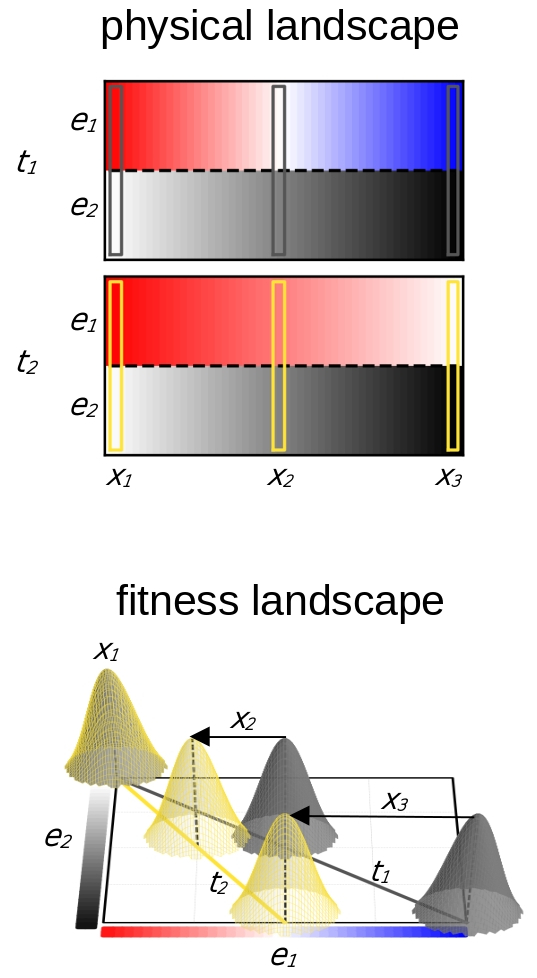
\includegraphics[width=.8\linewidth]{pub/figs/FIG_1_conceptual.jpg}
    \caption{Conceptual model of adaptation to climate change. Above: Stacked, horizontal cross-sections of our square simulation landscape, shown for the shifting environmental gradient ($e_{1}$, blue-red color ramp) and the stable gradient ($e_{2}$, white-black color ramp), both before climate change ($t_{1}$) and after ($t_{2}$). Below: Bivariate fitness landscape of the traits adapted to the shifting and stable gradients, on axes $e_{1}$ and $e_{2}$, respectively. Three example positions along the bivariate gradient ($x_{1}$, $x_{2}$, $x_{3}$) are delineated by thin vertical boxes on the physical landscape, both before climate change (gray) and after (yellow), and their corresponding fitness peaks are shown as color-matched kernels located along color-matched lines of the fitness optima that exist on the physical landscape before ($t_{1}$) and after ($t_{2}$) climate change. Shifts in local fitness peaks are shown as labeled arrows ($x_{2}$, $x_{3}$); the environment at the far left of the physical landscape does not change, so $x_{1}$'s fitness peaks are overlapping and have no shift, whereas the environment at the far right of the physical landscape experiences the maximal rate of change, which is reflected in the shift in $x_{3}$'s fitness peaks. Note that fitness peaks are stylized and truncated for ease of depiction; in our simulations, fitness decreases as a linear function of an individual's distance from its phenotypic optimum, rather than the truncated Gaussian function depicted here.}
\label{fig:fig_1}
\end{figure}


We use our simulations to test a series of hypotheses about the influence of genomic architecture 
on multivariate adaptation under climate change. First of all, we hypothesize that up-gradient 
gene flow is higher under climate change than in the null simulations under all 
scenarios, but that gene flow contributes least to adaptation in lower-linkage, 
high-polygenicity scenarios. This is because we expect gene flow to always have
at least some adaptive value, but expect low-linkage, high-polygenicity architectures 
(i.e., 'dispersed' architectures \cite{yeaman_review}) to exhibit quick \textit{in situ}
restructuring of allelic covariance among many small-effect alleles, akin to adaptation 
under transient genetic architectures, driving phenotypic shifts that are not maladaptive 
with respect to the stable gradient. Secondly, we hypothesize that stronger linkage 
and higher polygenicity will reduce a population's adaptive capacity under climate change
(i.e., will result in greater reductions in population size and mean fitness
and more persistent maladaptation), because both conditions require longer expected
wait times for the emergence of recombinant haplotypes that push phenotypes
away from their pre-change fitness peaks. Finally, we hypothesize that higher redundancy
facilitates adaptation to shifting gradients, much as it does on stable gradients 
\cite{barghi_redundancy,manceau,yeaman_amnat}, resulting in smaller reductions 
in population size and mean fitness than in our low-redundancy scenarios.




\section*{Results}

\subsection{Hypothesis 1: Gene flow}
As expected, up-gradient gene flow was always at least slightly higher
(and conversely, maladaptive downslope gene flow supressed) 
under climate change than in paired null simulations (\ref{fig:fig_2}).
However, contrary to our expectation we found that the amount of up-gradient gene flow
was negatively correlated with the level of linkage.
Polygenicity had the strongest overall effect on the amount that up-gradient gene flow contributes to adaptation:
with the exception of the low-redundancy, independent-linkage scenarios,
moderate and high polygenicity scenarios had much lower up-gradient gene flow
than did low-polygenicity scenarios. 
Interestingly, moderate-polygenicitiy scenarios consistently showed the least upslople gene flow,
though differences between moderate- and high-redundancy scenarios were mostly minimal.

\begin{figure}
\centering
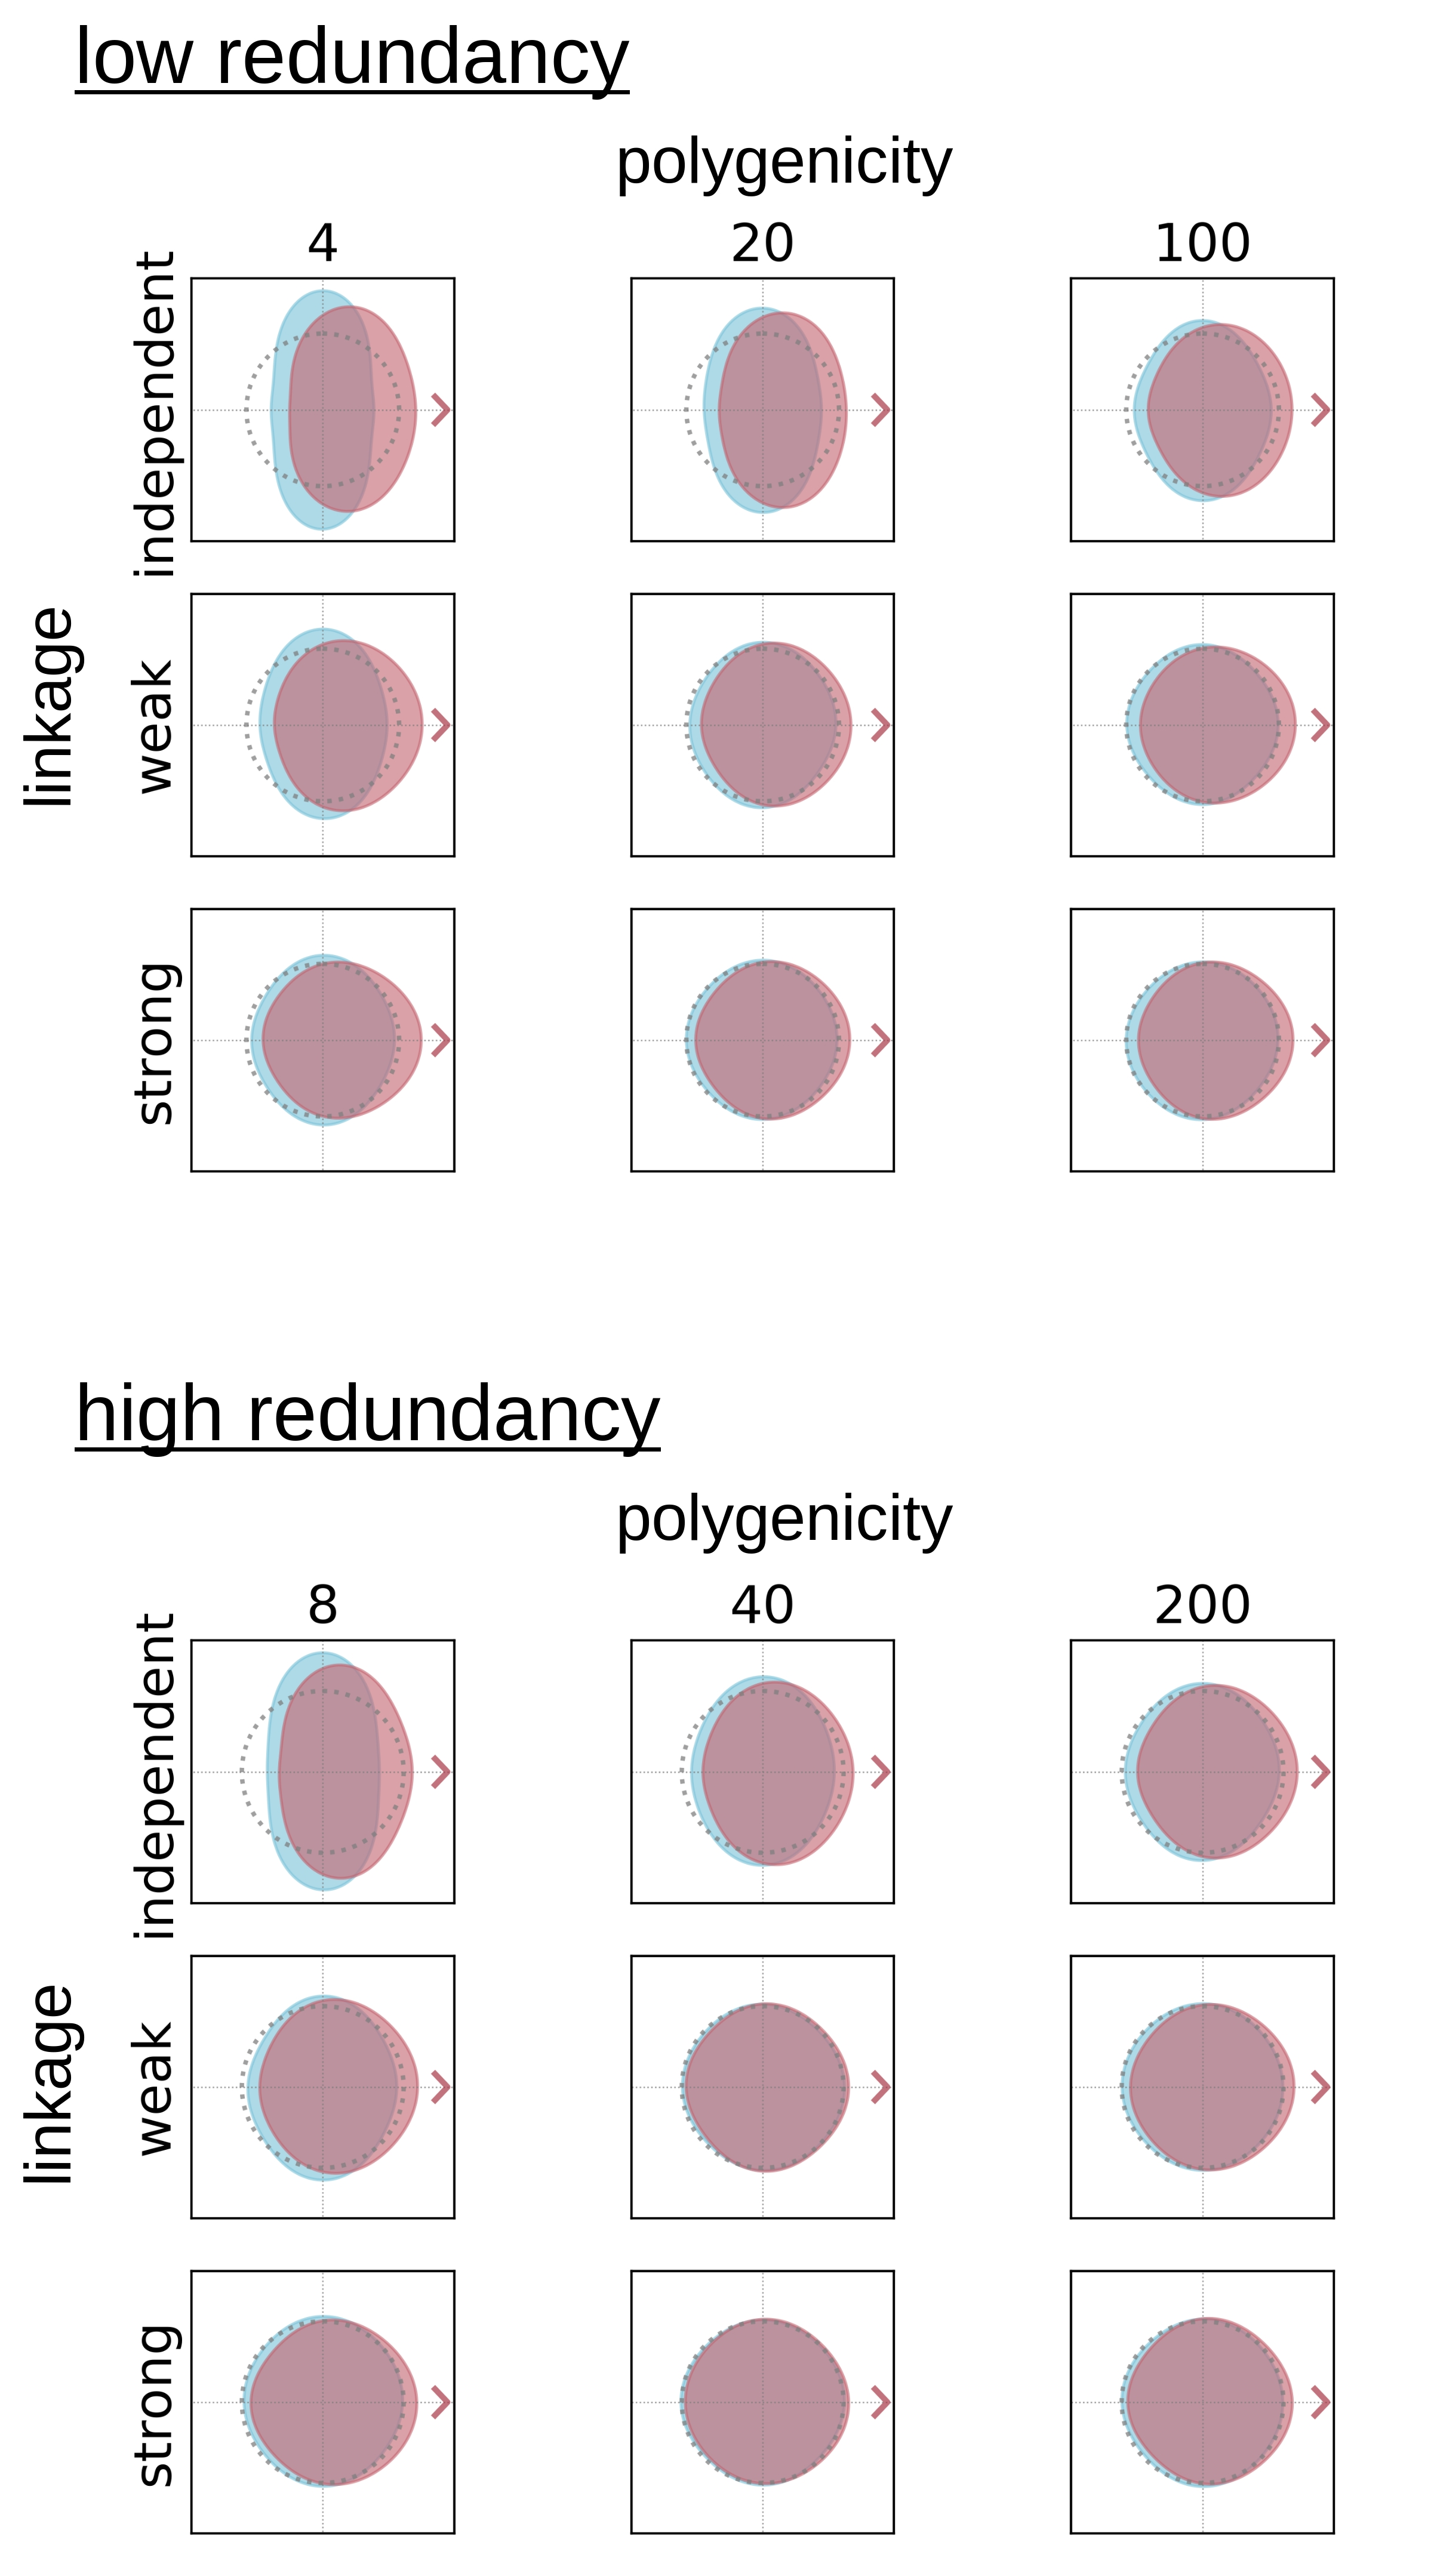
\includegraphics[width=.8\linewidth]{pub/figs/FIG_2_gene_flow.jpg}
    \caption{Comparison, across all 18 scenarios, of the distributions of gene-flow directions during the climate change period. Scenarios are organized into top and bottom sections for low and high redundancy, with rows in each section representing levels of linkage and columns representing polygenicity. Main scenarios (red) are compared against null scenarios (blue). Compass labels indicate directions of gene flow as it would be observed from a bird’s-eye view of the simulated landscape, with rightward (i.e., `up-gradient') gene flow moving in the same direction as the shifting environmental gradient, and with upward and downward (i.e., `on contour’) gene flow being perpendicular to the environmental gradients. Down-gradient gene flow is expected to be maladaptive under all scenarios, explaining why it is universally suppressed relative to the null results. There is a general trend toward increasing on-contour gene flow and decreasing up-gradient gene flow with increasing strength of linkage and increasing number of loci per trait..
}
\label{fig:fig_2}
\end{figure}


\subsection{Hypothesis 2: Linkage and polygenicity}
As expected, null simulations showed no change in mean fitness (\ref{fig_2}),
population size(\ref{fig_s2}), or phenotypic distribution (\ref{fig_s3}),
whereas climate change caused the maladaptation predicted under basic theory
\cite{aitken_whitlock},
decreasing population size and mean fitness and shifting phenotypic distributions (\ref{fig_4}).
Our main simulation results lend mixed support to our second hypothesis.
The magnitude of the demographic impacts of climate change was positively
correlated with the level of linkage across scenarios.
However, the effect of polygenicity
was more complex, with demographic effects being smallest at moderate polygenicity,
moderate at low polygenicity regardless of redundancy and at high polgenicity when redundancy was high,
but very large at high polygeniciy and low redundancy (\ref{fig:fig_3}, \ref{fig:fig_s2}).
Indeed, demographic decline was so strong at low redundancy and high polygenicity
that adaptive capacity was effectively outstripped: demographic decline persisted throughout
the climate change period, with little indication of evolutionary rescue
(i.e., stabilization and rebound) occurring until the artificial post-climate-change period.
The collapse of adaptive capacity in these scenarios
low is also visible in the low-redundancy, high-polygenicity plots in \ref{fig:fig_4}
(\textit{cf.}\ref{fig:fig_s3}),
which show much greater maladaptation (i.e., much larger red areas of phenotypic shortfall),
than the small amount that occurs in all other scenarios.
The low-redundancy, high-polygenicity, strong-linkage scenario had such low adaptive capacity
that mean fitness declined by XXXXXX\% on average (from XXX to XXX),
mean population size declined by XXXXX\% on average (from ~XXXXXX to ~XXXX individuals),
and the simulated population went locally extinct in the rightmost, fastest-changing portion of the landscape.
This is visible in \ref{fig:fig_4} as the disappearance of population density in the portion
of the post-climate change phenotypic space corresponding to that region of the landscape,
but is more clearly visible in the before-after population density maps in \ref{fig:fig_s4}.

\begin{figure*}[\sidecaptionrelwidth][t]
\centering
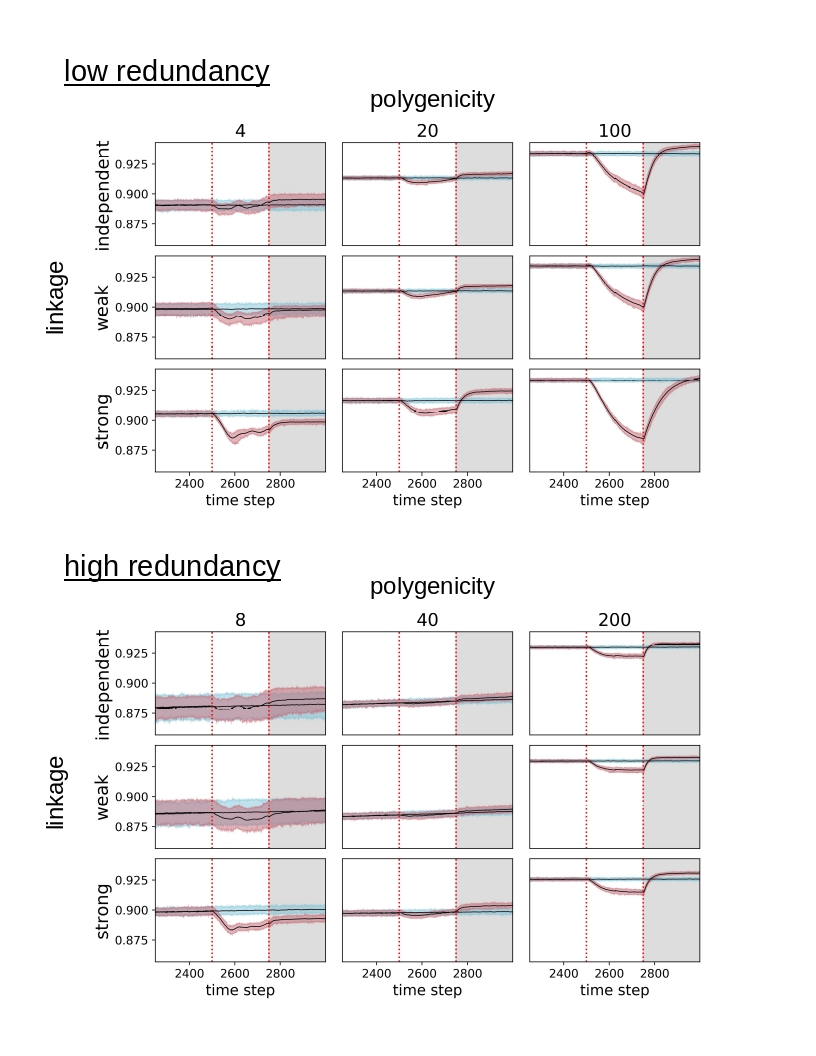
\includegraphics[width=17.8cm]{pub/figs/FIG_3_fit_over_time.jpg}
\caption{Left: Mean fitness dynamics for all scenarios during the 250 time steps before the climate change period and the 250 time steps during it (with the two periods divided by a red, dashed vertical line marking the onset of the climate change period). Scenarios are organized as in \ref{fig_2}: top and bottom sections for low and high redundancy, with rows in each section representing levels of linkage and columns representing polygenicity. Right: Comparison of climate change-driven changes in mean fitness across scenarios. Null scenarios are plotted on the left in blue, and main scenarios are plotted on the right, in red. Within each plot, scenarios are divided by the number of loci per trait (x-axis) and by the strength of linkage (shade, with darker hues representing stronger linkage). Asterisks above each box indicate level of significance (*=0.1, **=0.05, ***=0.005).}
\label{fig:fig_3}
\end{figure*}

\begin{figure*}
\centering
% NOTE: MAY NEED TO ADJUST THIS FIG TO FIT PNAS FORMAT, IF EVENTUALLY WE AND GET ACCEPTED THERE
%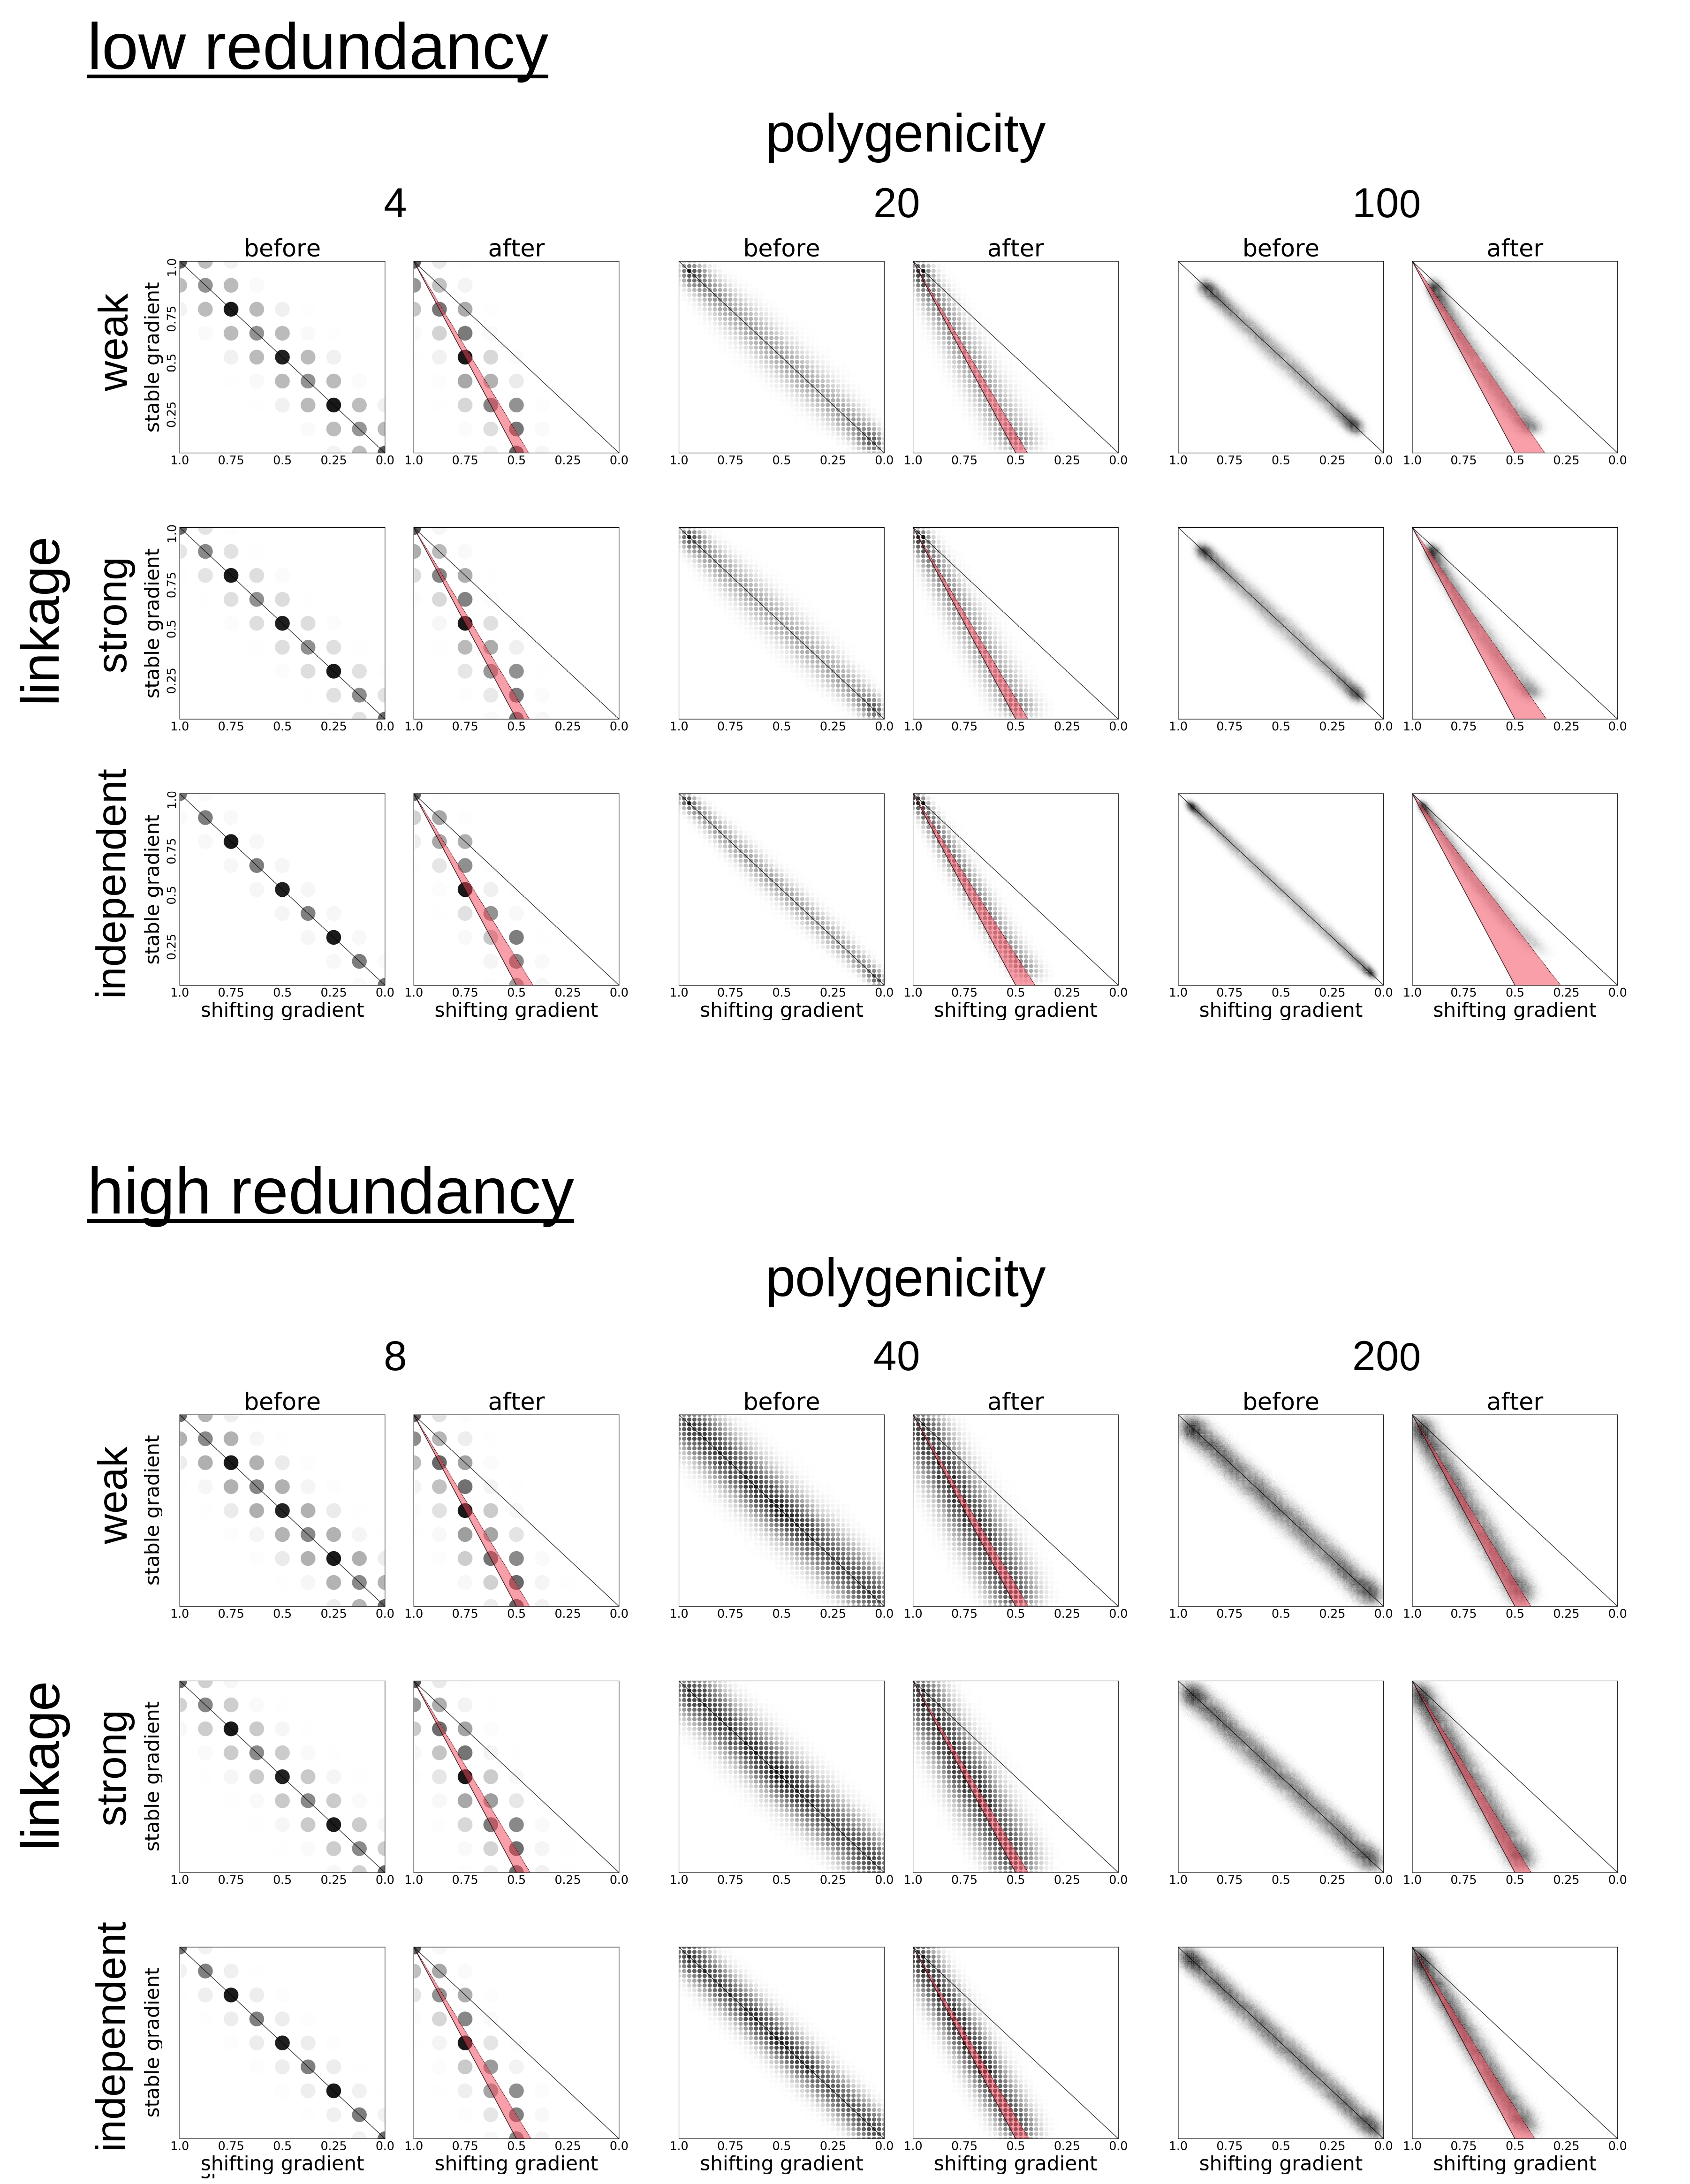
\includegraphics[width=17.8cm]{pub/figs/FIG_4_phenotypic_shift.jpg}
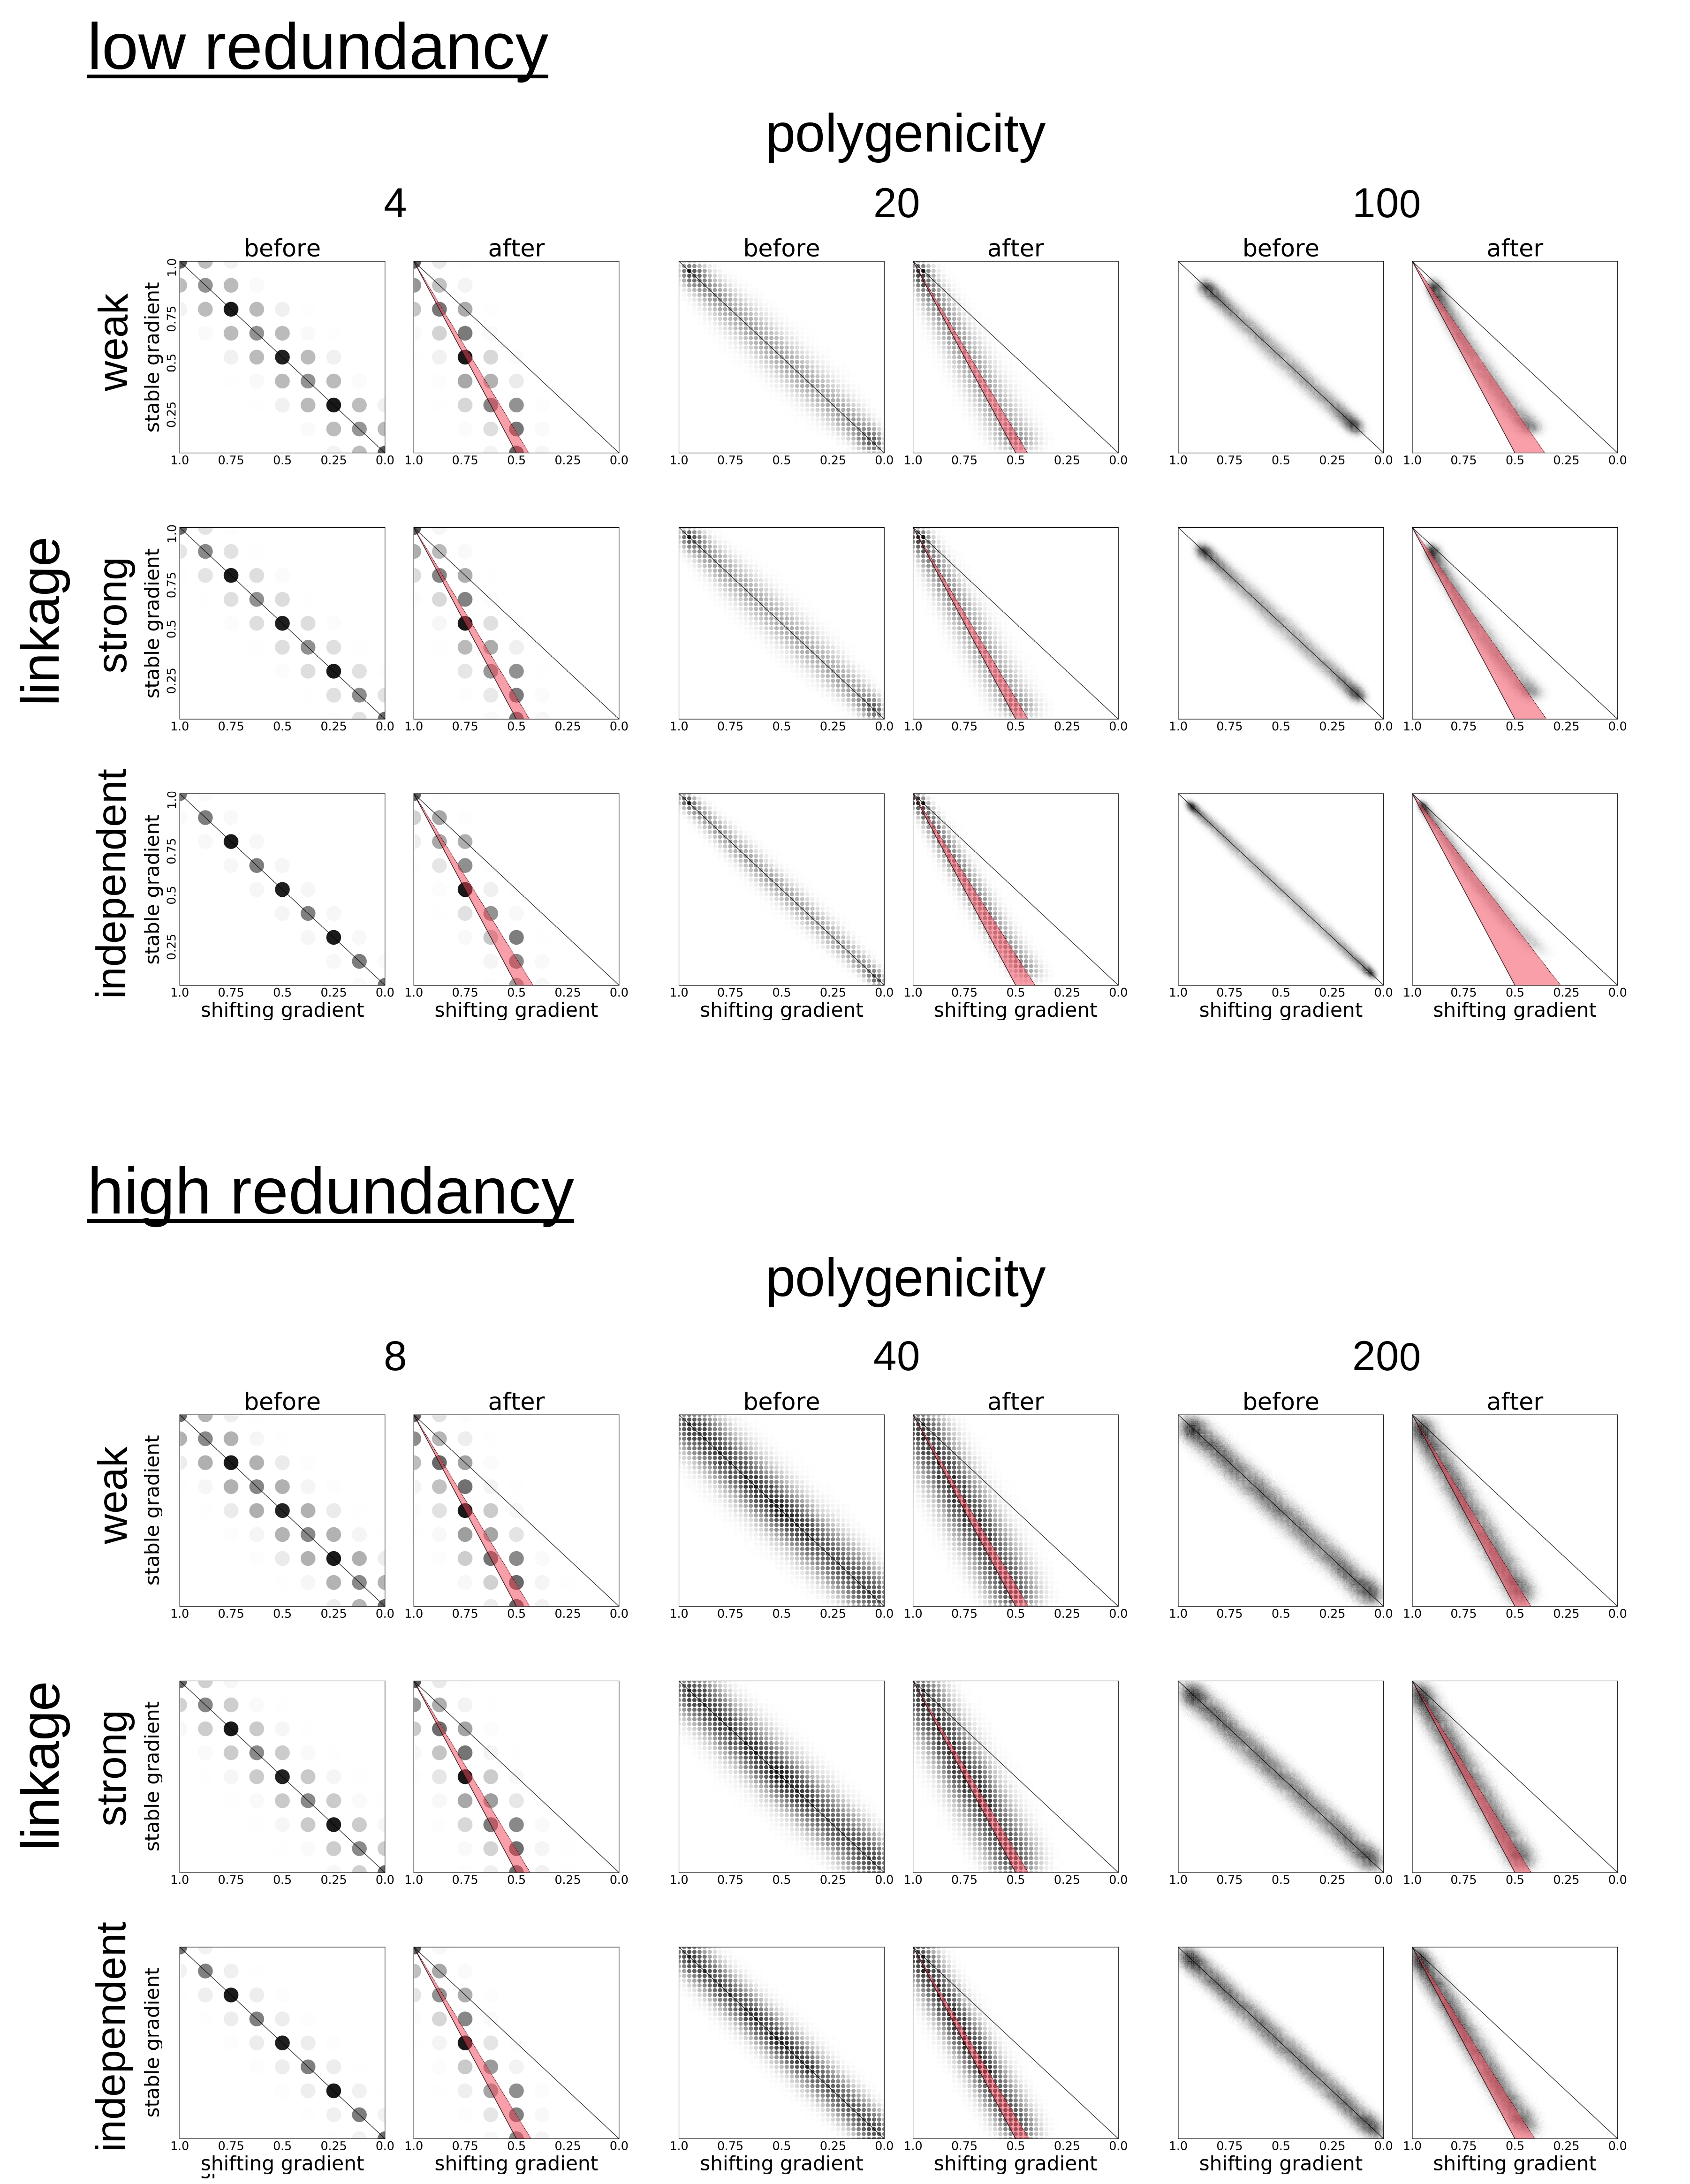
\includegraphics[width=15.8cm]{pub/figs/FIG_4_phenotypic_shift.jpg}
\caption{Comparison, across all 18 redundancy scenarios, of the observed versus expected phenotypic shift during the climate change period. Scenarios are organized as in \ref{fig_2}: top and bottom sections representing low and high redundancy, with rows in each section representing levels of linkage and columns (in before-after pairs) representing polygenicity. For each scenario, the left ('before') scatterplot shows the distribution of individuals’ bivariate phenotypes before climate change begins, whereas the right ('after') scatterplot shows how the distribution has shifted by the end of the climate change period. The trait adapted to the shifting environmental gradient is distributed along the x axis, and the trait adapted to the stable gradient is distributed along the y axis. Scatterplots depict multi-model ensemble results for each scenario. The size and opacity of each point represents the number of individuals exhibiting that bivariate phenotype. (Note that the gridded arrangement of the points in each scatterplot is a function of the number of loci per trait which, because locus effect sizes are fixed, directly determines the set of attainable, evenly-spaced, discrete phenotypic values. Because fewer loci per trait yields fewer possible phenotypes, individuals are grouped into fewer, larger phenotypic bins in the 4- and 20-locus scenarios.) Solid black lines delineate the shift in the phenotypic distributions’ central tendencies that is expected to take place during the cimate change period, dotted black lines depict the observed (OLS-fitted) phenotypic distributions’ central tendencies at the ‘during’ and ‘after’ time steps, and translucent red wedges depict the differences between the expected and observed distributions (i.e., ‘phenotypic shortfall’, the response variable in our statistical tests).
}
\label{fig:fig_4}
\end{figure*}
 

\subsection{Hypothesis 3: Redundancy}
Our third hypothesis was fully supported by our results: High-redundancy scenarios showed
consistently smaller demographic impacts of climate change and higher adaptive capacity
than their low-redundancy comparators (\ref{fig:fig_2}, \ref{fig:fig_s2}).
As mentioned above, this was especially notable in the high-polygenicity scenarios,
which did not show not show evidence of demographic rebound during climate change.
This is not to say that adaptation successfully occurred in all other scenarios though:
fitness and population declines stabilized but did not rebound
in high-redundancy, high-polygenicity scenarios (\ref{fig:fig_2}, \ref{fig:fig_s2}).



\section*{Discussion}

Current thinking about evolutionary responses to climate change
frequently starts from a simplified mechanistic model in which
adaptation is facilitated by up-gradient gene flow.
This model not only serves as the conceptual basis for research,
but also as the inspiration for some climate-smart
approaches to biodiversity management
(e.g., assisted gene flow; \cite{aitken_whitlock}).
Yet the validity of the model under different
genomic architectures has rarely been tested --- let
alone under the complex multivariate architectures we simulate here.
Our study finds first-order, empirical support for this
model across the range of genomic architectures explored,
given that up-gradient gene flow during climate change
is equal or greater under all simulation scenarios
as compared to static-environment null simulations.
However, our results also suggest a major caveat:
Polygenicity, and to a lesser extent linkage,
can constrain the extent to which up-gradient
gene flow contributes to adaptation under environmental change.
In the case of linkage, our results contradicted our first hypothesis,
perhaps because lower recombination between both traits'
genes makes up-gradient gene flow more maladaptive,
despite creating larger-effect clusters of non-neutral loci.
Given the plausibility of the range of genomic architectures we simulate
\cite{barghi_polygenic,boyle,rockman,savolainen,sella,bomblies},
these results raise the compelling
possibility that up-gradient gene flow, while unlikely
to be maladaptive, could nonetheless prove
ineffectual for supporting adaptation in many systems.
This poses important questions for subsequent research:
How applicable are our low-polygenicity results to real-world
systems --- i.e., how often does species' climatically-adaptive
standing genetic variation include
rare, large-effect alleles that might predominate in
evolutionary responses to climate change?
And how can such systems be distinguished from high-polygenicity systems,
so as to redirect management funds from assisted gene flow
to more apt strategies (e.g., marker-assisted selection; \cite{muranty}) as needed?


Aside from gene flow patterns, the population dynamics of evolutionary responses
to climate change are also rarely considered in the context of genomic architecture.
Our results show that neglecting genomic architecture
can lead to overlooking important evolutionary contingencies,
whereas accounting for them can help extend current theory.
First, our models suggest that maladaptation and demographic decline
can be augmented by strong linkage between non-neutral loci,
especially under high polygenicity. 
In the most extreme case, high polygenicity and low redundancy
combine to drive dramatic and persistent declines,
and even local extinction when linkage is strong.
This was unexpected in light of previous work reporting that genetic architectures composed
of many genes of small effect (i.e., 'dispersed' genetic architectures) produce stable,
resilient phenotypic clines despite transient genotypic composition \cite{yeaman_amnat,yeaman_review},
and thus that species with such architectures
could exhibit rapid local adaptation \cite{aitken_yeaman}. 
We still expected evolutionary responses to climate change
to be slower in these scenarios,
because natural selection is less effective on smaller-effect alleles
and because high linkage leads to longer expected wait times to the generation
of novel, adaptive recombinants, but we did not expect
to see a complete inability to adapt.
The fact that high genotypic redundancy reduces demographic decline,
not just in these but across all scenarios,
not only echoes the recently recognized importance of redundancy
as a driver of population-genetic outcomes in polygenic systems
\cite{laruson,yeaman_review},
but also presents a possible mechanism to be explored
in real-world populations living at species' colder range edges.
Much like the local populations in the rightmost region of our low-redundancy scenarios,
these populations could already be at the edge of the phenotypic space defined by
standing genetic variation, such that local selection would be directional,
segregating redundancy (\textit{a la} \cite{laruson}) correspondingly low,
adaptive capacity lacking, and extinction vulnerability substantial.
However, if cold range boundaries are not bioclimatically determined then
these populations could be more similar to our high-redundancy scenarios:
selection would be balancing rather than directional,
segregating redundancy substantial, and thus adaptive capacity more robust.

Our simulations exhibit other intriguing patterns
that indicate theoretical ambiguities that could benefit from further work.
First, our results add an interesting complication
to the theoretical generality that recombination can be deleterious
in situations of clinal adaptation
with gene flow because it disrupts the association between adaptive loci 
underlying a single trait \cite{tigano}.
While this may apply in the special case of a single-trait 
adapted to a single gradient,
we find that it may change under other realizations of the 
generalized model of $n$ traits adapted to $n$ gradients:
In our two-trait, two-gradient model, given that the gradients decouple
and novel environments emerge,
recombination appears advantageous.
This is because, despite the fact that recombination disrupts the association between
adaptive loci for the shifting gradient's trait, preventing the
generation of larger-effect gene clusters,
it also dissociates those loci from the loci underlying
the stable gradient's trait, for which gene flow could be maladaptive.
In other words, recombination facilitates adaptive gene flow
by providing escape from the genetic conflict between
two separate and complex genetic architectures.
 
Second, the minimal demographic decline
in our moderate-polygenicity models,
contrasts with previous work reporting that adaptation
to a gradient is most effective under either
concentrated or dispersed genomic architectures.
This discord may be attributable to the
difference in timeframes between adaptation to a univariate environmental gradient
and adaptation to a decoupling, multivariate gradient.
Adaptation to a single, static gradient can proceed gradually,
so may either favor large-effect alleles or allele-clusters in the long haul
\cite{yeaman_amnat,yeaman_review},
once they have arisen by mutation, recombination, gene flow, or a combination thereof,
or dispersed architectures 
\cite{burger,kondrashov,yeaman_review,yeaman_whitlock}
in temporally fluctuating environments.
However, the sudden onset of persistent environmental change 
in a population that is already locally adapted triggers a 'race against time', 
and it may be that the genetic architectures with
optimal adaptive capacity are 'middle ground' architectures that comprise
freely recombining loci with small-enough effect sizes to avoid large
sudden declines in fitness from migration load,
but with large enough effect sizes to avoid the long wait times necessary
for recombination to cluster many adaptive loci into larger-effect haplotypes.
If this is true it would suggest an inherent tension between the architectures that
might be expected to evolve in locally adapted populations prior to climate change
and those most likely to facilitate adaptation to change.
Further research, both empirical and theoretical,
may help determine the conditions under which this tension
may be especially strong and thus may deflate
populations' adaptive capacity.
 
A major challenge in simulation-based research is the complexity of the high-dimensional 
parameter space that could be explored.
Informative studies can be constructed by focusing on a small set of
key parameters while holding others at reasonable values, as we have done here.
This nonetheless leaves unexplored a number of secondary parameters
that can have non-negligible influence over the complex ecological phenomena of interest.
In the case of evolutionary responses to climate change,
a number of these provide areas for future research, including:
population size, a key determinant of the relative strengths of drift
and natural selection \cite{murray} and of the wait time to emergence of
recombinant haploytpes \cite{christiansen}, among other important dynamics;
movement behavior, a key factor embedded in the rudimentary
migration-selection dynamics that lie at the heart of models like ours
\cite{wright,haldane,barton};
allelic effect size distributions \cite{orr},
which are omitted here in favor of a single fixed effect size but would
help clarify evolutionary tendencies when loci of varying effect sizes
are simultaneously subject to selection;
and the structure of the environment,
including the geometries, slopes, and orientations of gradients
(e.g., \cite{benes}) and their rates of change.
A number of other more complex evolutionary aspects could also be explored 
through a similar modeling framework, including 
pleiotropy \cite{thompson} and epistasis,
hybridization CITE, and life history variation.
Finally, important and conservation-relevant insight could emerge from the 
integration of other dimensions climate change ecology, including range shifts 
\cite{weiss-lehman}, plasticity \cite{chevin},
and range-wide variation in population density \cite{aitken_whitlock}.

Our study not only provides various insights into the nature
of polygenic adaptation to multivariate environmental change,
but also emphasizes the theoretical and applied importance
of this neglected area of research.
It corroborates some principles derived from previous theory
of local adaptation to static, univariate environments, but also suggests
ways in which multivariate environmental change extends
or complicates current theory.
Much work remains to be done to better understand and predict
evolutionary responses to climate change,
and our work points toward fruitful next steps.



\matmethods{

\subsection*{Simulation}

We built all of the simulations for this study using \texttt{geonomics} \cite{terasaki_hart},
a Python \cite{rossum} package for
creating forward-time, agent-based, continuous-space landscape genomic simulations 
using arbitrarily complex life histories, environments, and environmental change 
scenarios. We created a base scenario for our set of simulations
by creating a template parameters file featuring
a species with two traits, each of which experiences 
selection on the basis of a different environmental variable (using the \texttt{geonomics.make\_parameters\_file} command).
Both environmental variables are modeled as linear, horizontal gradients
that initially span environmental values from 1 to 0, left to right.
Individuals' fitness is a function of the difference between their local
environmental values and their phenotypes, which are determined by the
additive effects of multiple loci (i.e., without pleiotropy or epistasis) ---
a reasonable approximation of many traits of interest in real populations \cite{sella}.

Each simulation starts with a neutral burn-in period, ended by \texttt{geonomics}' tests
of temporal and spatial population stability, then runs for 2500 time steps
non-neutral evolution, generating a pattern of local adaptation to the initial environment.
After that, one of the environmental layers undergoes a change 
event in which the gradient’s values change stepwise over a period of 250 time steps,
resulting in a final gradient that spans values from 1 to 0.5, left to right.
This creates a scenario in 
which the two environmental variables become decoupled, leading 
to the emergence of novel environments (i.e. sites occupying new vectors in 
two-dimensional environmental space).
The purpose of this is to emulate a common 
phenomenon under climate change: the decoupling of multivariate environmental gradients,
leading to the emergence of novel climates
\cite{williams_novel_climates,williams_projected_novel_disappearing,fitzpatrick_climate_novelty_forecasts}.
Importantly, this landscape arrangement generates heterogeneous rates of climate change,
with the rate ranging from 0 at the leftmost edge to $\frac{0.5}{250 time steps}$ at the rightmost edge.
This complicates interpretation of our results,
but less so than in an alternative scenario
with spatially homogeneous rates of change,
which would generate an artefact of range expansion
whose genomic signal would be superimposed on that of
climate change adaptation.
This latter approach is also of interest,
and may be explored in future work,
but the approach we chose here allows us
to best isolate the evolutionary dynamics
resulting from the components of genetic architecture
that define our scenarios and hypotheses.

Next we wrote a custom Python script that reads the template \texttt{geonomics}
parameters file, edits any parameters that vary 
across our scenarios, instantiates a model, runs a fixed number of iterations 
of that model, and outputs simulated genetic and other data. 
Our parameters of interest, and the values we assigned them, are:
 - the number of loci underlying each trait (parameter \texttt{n\_loci}):
   - low = 5
   - moderate = 20
   - high = 100
 - the linkage between neighboring loci, i.e., the homogeneous recombination rate (parameter \texttt{r}):
   - unlinked = 0.5
   - weak linkage = 0.05
   - strong linkage = 0.005
 - the amount of genotypic redundancy (parameter \texttt{n\_loci}):
   - low: the values specified above produce many-to-one genotype-phenotype mappings at intermediate phenotypes, declining to one-to-one mappings at extreme phenotypes
   - high: doubling of the values produces many-to-one mappings across all phenotypes between 0 and 1, inclusive (i.e., all phenotypes matching environmental values somewhere on the landscape).
The full factorial combinations of the chosen values of those parameters generate the set
of simulation scenarios depicted in the tabular arrangments of figures
\ref{fig:fig_2}, \ref{fig:fig_3}, \ref{fig:fig_4}, \ref{fig_fig_s2}, \ref{fig_fig_s3}, and \ref{fig_fig_s4}.
We used that script to run a set of batch jobs on the 
savio3 partition of UC Berkeley’s Savio system (each node has 96 GB RAM and 32, 
2.1-GHz Skylake processors). For each scenario, we ran a total of 100 iterations of 
the scenario of interest, featuring a 250-time-step climate change period (henceforth, 
the ‘main’ scenarios), and 100 iterations of a paired null scenario without natural 
selection (henceforth, the ‘null’ scenarios). 
Given that \texttt{geonomics} is a complex simulation framework, it features numerous other 
parameters, which we set at reasonable default values.
For the complete set of parameters and the values 
assigned to them across all models
(as well as green-highlighted notes denoting runtime and genomic-architecture
parameter overridden by the main simulation scripts), see Appendix 1.

Using a combination of internal \texttt{geonomics} functions and custom Python code, we 
designed a set of data outputs from each model run that would allow us to test our 
series of hypotheses. We saved tables of individuals’ locations and phenotypes at both
the beginning and the end of the climate change period. We also saved time 
series of population size, mean fitness, and mean phenotype of the trait adapted to 
the shifting gradient. We gathered this data at every time step, from 250 time steps 
before the onset of climate change, through the 250 time steps of the event, and 
continuing until 250 time steps after climate change completed.
The final 250 time steps after climate change are unrealistic, but are useful
for elucidating the nature of the changes that persisted to the end of the climate change period;
we refer to this period as the 'post-change period'.

We also saved data on the vector directions of all gene flow during the 
climate change period, extracted from the spatial pedigrees stored in the
\texttt{tskit} \cite{kelleher} data structures.
From that full set of gene flow data we calculated a pair of measures
of gene flow directionality,  which we refer to as ‘rightness’ (i.e., up-gradient 
directionality) and ‘up-downness’ (i.e., on-contour directionality). These were 
calculated as:

$Rness = \frac{\sum\limits_{i}^{n}\cos\theta}{n},\ \cos\theta\geq0$,

$UDness = \frac{\sum\limits_{i}^{n}|\sin\theta|}{n}$,

where angles are expressed counterclockwise from the right.
We ignored leftward gene flow because it was expected to be low irrespective 
of scenario, given that it would oppose the environmental shift so would be largely maladaptive.
DOUBLE-CHECK THE SENTENCE BELOW
We also saved a subsample of the full set of gene flow 
direction data by keeping all data pertaining to two randomly chosen loci that had 
positive effects on the trait adapted to the shifting environmental gradient. We 
restricted our sample in this way both to focus on loci expected to facilitate 
adaptation to increasing environmental values and thus to shift upslope, and to 
provide equal sample sizes across scenarios in downstream analysis (which was 
constrained to the number of positive-effect loci present in the four-locus-per-trait 
scenarios, i.e. two). 

\subsection*{Analysis}

We analyzed all 18 scenarios' and all 100 iterations' data
using visual summaries and companion statistical tests.
All analysis and visualization was produced using custom scripts written in 
Python and R \cite{r_core_team}.

To test our first hypothesis about gene flow,
we first produced a visualization of the directional 
distributions of gene flow in all 18 scenarios, comparing between main
and null scenarios (\ref{fig:fig_2}).
To create this visualization, we gathered directional data
from each simulation for a random 
sample of the gene flow that occurred during the climate change event, using 
\texttt{geonomics}' integration with \texttt{tskit} \cite{kelleher}, which allows for temporal 
subsetting and output of the information contained the full spatial pedigree of a 
simulated population. We then fitted a mixture of 4 von Mises distributions to that data, 
yielding 12 parameter estimates defining each simulation's fitted mixture distribution. For each of 
the 18 scenarios, we then plotted the probability density function 
described by the means of all length-12 vectors of fitted parameters. We did this 
separately for null scenarios and for main scenarios, then overlaid the null (in blue)
and main (in red) results, providing a summary depiction of the nature of gene flow within each 
main scenario as compared to its null expectation.
Finally, we ran two-way ANOVAs of 
rightness and up-downness (with Bonferroni correction for multiple testing), 
to test the null hypotheses that the values of both directional metrics
had no statistical relation to our genomic architecture parameters
of interest (polygenicity, linkage, and genotypic redundancy),
followed by \textit{post hoc} Tukey's honest significant difference (HSD) tests
to determine the nature of the relationship between those metrics and our
genomic architecture parameters of interest.
As a comparator, we also ran this analysis for our null data.

To visually assess our second and third hypotheses, we created a series of
plots comparing climate change-driven demographic shifts
and maladptation across all 18 scenarios and between null and main moels.
First, we plotted the 
null and main trajectories of two demographic
metrics --- mean fitness and population size --- in 
each of our 18 scenarios. For each scenario and metric, and 
for both main and null models, we created ensemble datasets by combining all 100 
iterations’ output time series of the metric,
then derived summary time series by calculating each time step's
100-iteration mean and 5th and 95th percentiles.
We plotted the resulting summary time series in \ref{fig:fig_3} (mean fitness)
and \ref{fig:fig_s2} (population size), with null results again shown in blue
and main results in red.
We plotted the metrics starting from 250 time steps before the climate change event
and running until 250 time steps after its completion, allowing us
to evaluate the onset, course, and aftermath of the demographic responses.
Additionally, we summarized all scenarios in a pair of box plots
(one plot for low genotypic redundancy, one for high),
with plots arranged by polygenicity along the x-axis,
colored blue or red to denote null or main results,
and shaded darker for increasing levels of linkage.

Next, to better understand changes in population size and distribution,
we mapped before-after comparisons of population density across all 18
main scenarios (\ref{fig:fig_s4}).
Each population density map is calculated as
the array of mean population densities at all cells on the landscape,
averaged across all 100 main simulations of the map's corresponding scenario.
Population densities are depicted as increasing from black to white, with
values standardized across the entire plot grid.

Finally, to visualize maladaptation, we created an identically-structured
grid of plots comparing each scenario's
mean phenotypic distributions before and after climate change,
including scatter plots of the density of individuals occuring across
two-dimensional trait space and lines and wedges depicting the average maladaptation
observed across each scenario's 100 iterations (\ref{fig:fig_4}).
We refer to the wedge as 'persistent maladaptation',
and we calculate it as the difference between: a.) the area 
within two-dimensional trait space that the population’s phenotypic distribution 
would have needed to shift through during the climate change event, so as to remain 
optimally fit to its environment, and b.) the observed area of phenotypic shift within
a scenario's 100 simulations.
(We qualify this metric as 'persistent' to emphasize that it does
not reflect transient maladaptation that arises but then
resides during the period of climate change, but rather reflects
only maladaptation that remains at the end of the climate change period.)
To measure this area, we first determined the triangular area between 
the expected central tendency lines of the optimal bivariate phenotypic distributions
before and after the climate change event;
these are unambiguously determined by the model parameterization, because
they are the lines connecting all of the discrete 
points in environmental space that occur on the pre- and post-change landscapes.
Then, for each model run, we used ordinary least squares (OLS)
to fit a central tendency line to the 100-iteration ensemble phenotypic distribution
observed at the end of the climate change event
(arithmetically fixing the y-intercept at the (1,1) point in phenotypic 
space, the unchanging phenotypic optimum at the leftmost extent of the landscape).
The area of the wedge between the expected and observed post-change central tendency
lines provides our measure of a scenario's persistent maladaptation.
We plot before and after scatter plots of the ensemble datasets
of individuals' two-dimensional phenotypes
(binned to a grid of regular points for interpretability, with points
shaded to depict relative densities of individuals).
We then overplot onto those scatter plots the central tendency lines of
the expected (dotted lines) and observed (solid lines) phenotypic distributions,
as well as the wedges of persistent maladaptation.
In \ref{fig:fig_s3} we produce the same plot as \ref{fig:fig_4},
but using data from null simulations to demonstrate that all differences
in maladaptation observed between scenarios were attributable to climate change,
and with blue translucent wedges showing the expected area of phenotypic shift
under each null scenario's corresponding main simulation, for reference.

To statistically test our second and third hypotheses,
we ran multi-factor ANOVAs on each of three response variables measuring
population-level changes during the climate change event ---
change in mean fitness, change in population size,
and persistent maladaptation --- with polygenicity,
linkage, and redundancy serving as genomic-architecture
ORDINAL OR CATEGORICAL??
factors.
For each ANOVA, we then used \textit{post hoc} HSD tests
to help determine the influence of explanatory variables,
treating the p-values of each explanatory variable,
in combination with the cross-scenario trends visible in
\ref{fig:fig_3}, \ref:{fig:fig_s2}, and \ref{fig:fig_4},
as tests of the components of our second hypothesis
(polygenicity and linkage) and third (redundancy).

} % end matmethods




\showmatmethods{} % Display the Materials and Methods section

\acknow{We thank A. Bishop, T. Dawson,  J. Frederick, N. Graham, M. Kelly, M. McElroy, E. Westeen, G. Wogan, and M. Yuan for feedback and guidance on various iterations of the simulations presented herein. We thank Berkeley Research Computing for providing access to the Savio computing cluster. We thank D. Ehrenfeld, N. Fefferman, M. Fitzpatrick, and L. Plough for cultivating an interest in conservation genetics. Lastly, we thank M. Terasaki Hart, C. Nemec-Hart, G. Hart, J. Hart, and M. Tylka for supporting and encouraging a lifetime of curiosity about nature, and C. S. aTunde Adjuah, B. Evans, R. Pérez Joglar, Y. Y. Ma, and J. Redman for the pleasant solitude. This work was supported by a Berkeley Fellowship (to D.E.T.H.) and by National Science Foundation grant DEB1845682 (to I.J.W.).}

\showacknow{} % Display the acknowledgments section

% Bibliography
\bibliography{terasaki_hart_ch2}

%%%%%%%%%%%%%%%%%%%%%%%%%%%%%%%%%%%%%%%
% TEMPORARY PLACE FOR SUPPLEMENTAL FIGS

\textbf{SUPPLEMENTAL FIGS:}


\begin{figure}
\centering
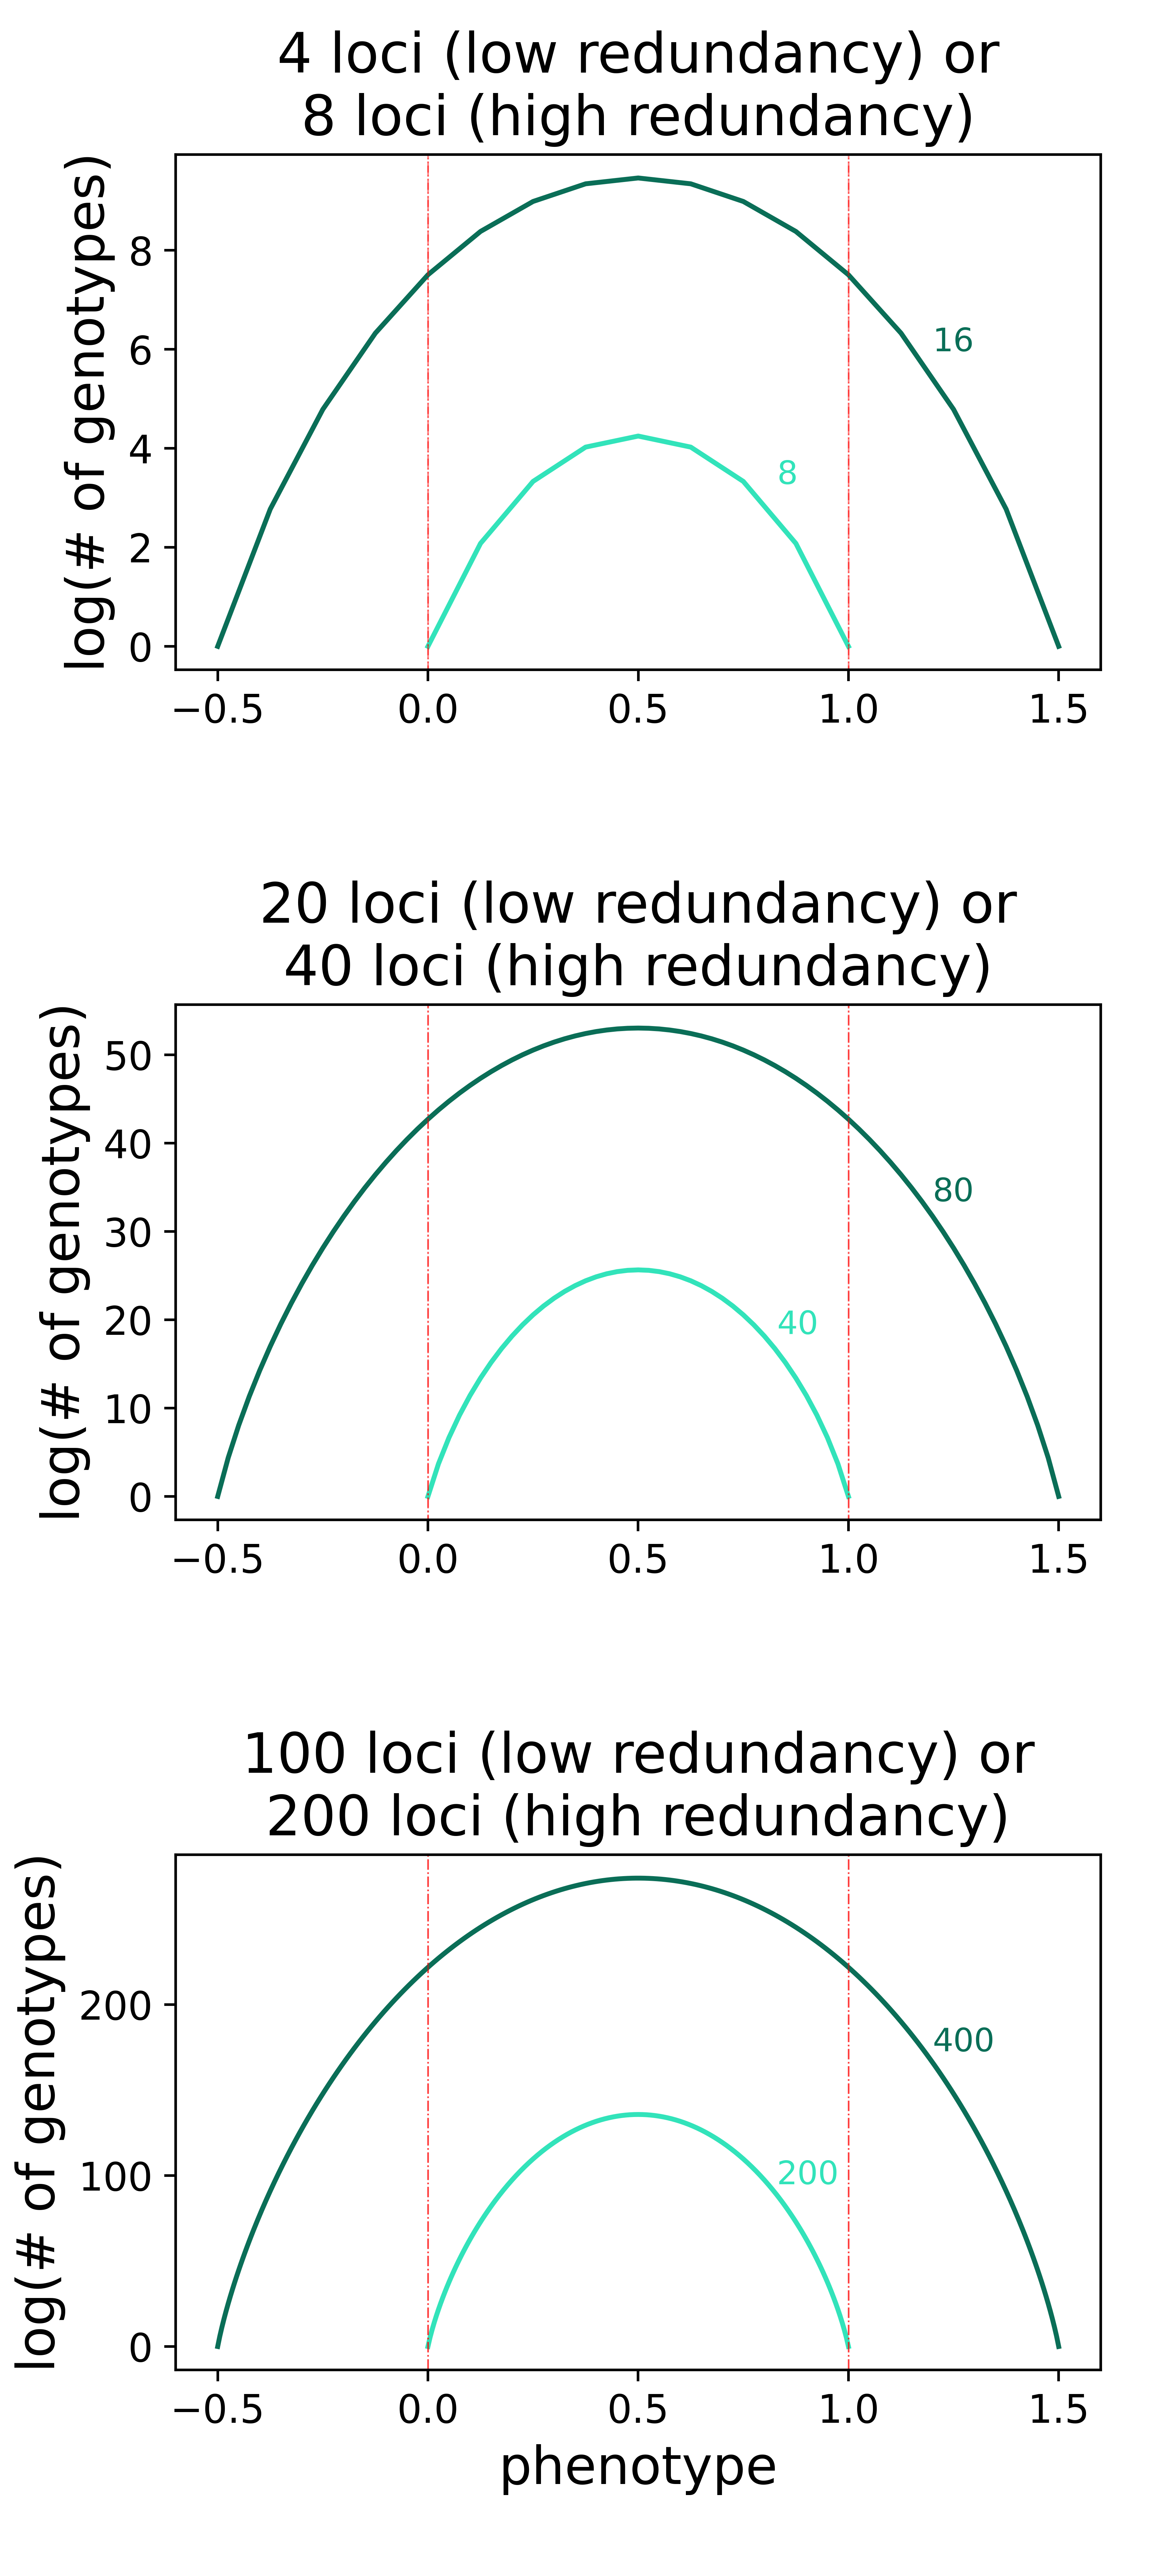
\includegraphics[width=.8\linewidth]{pub/figs/FIG_S1_redundancy.png}
\caption{Depiction of redundancy for all simulated polygenicity values. Phenotypic values are plotted along the x-axis, and the natural log of the number of genotypes that yield each phenotypic value is plotted along the y-axis. Polygenicities corresponding to low-redundancy scenarios are plotted and labeled in light teal, and those corresponding to high-redundancy scenarios in dark teal. The minimum and maximum environmental values on the landscape are represented by dotted vertical lines. The number of genotypes corresponding to each phenotype is calculated using a custom adaptation of Eqxn. ii, Box 1 in \cite{laruson}, implemented for a diploid species and fitted to the numerical conventions used by Geonomics.
}
\label{fig:fig_s1}
\end{figure}


\begin{figure*}[\sidecaptionrelwidth][t]
\centering
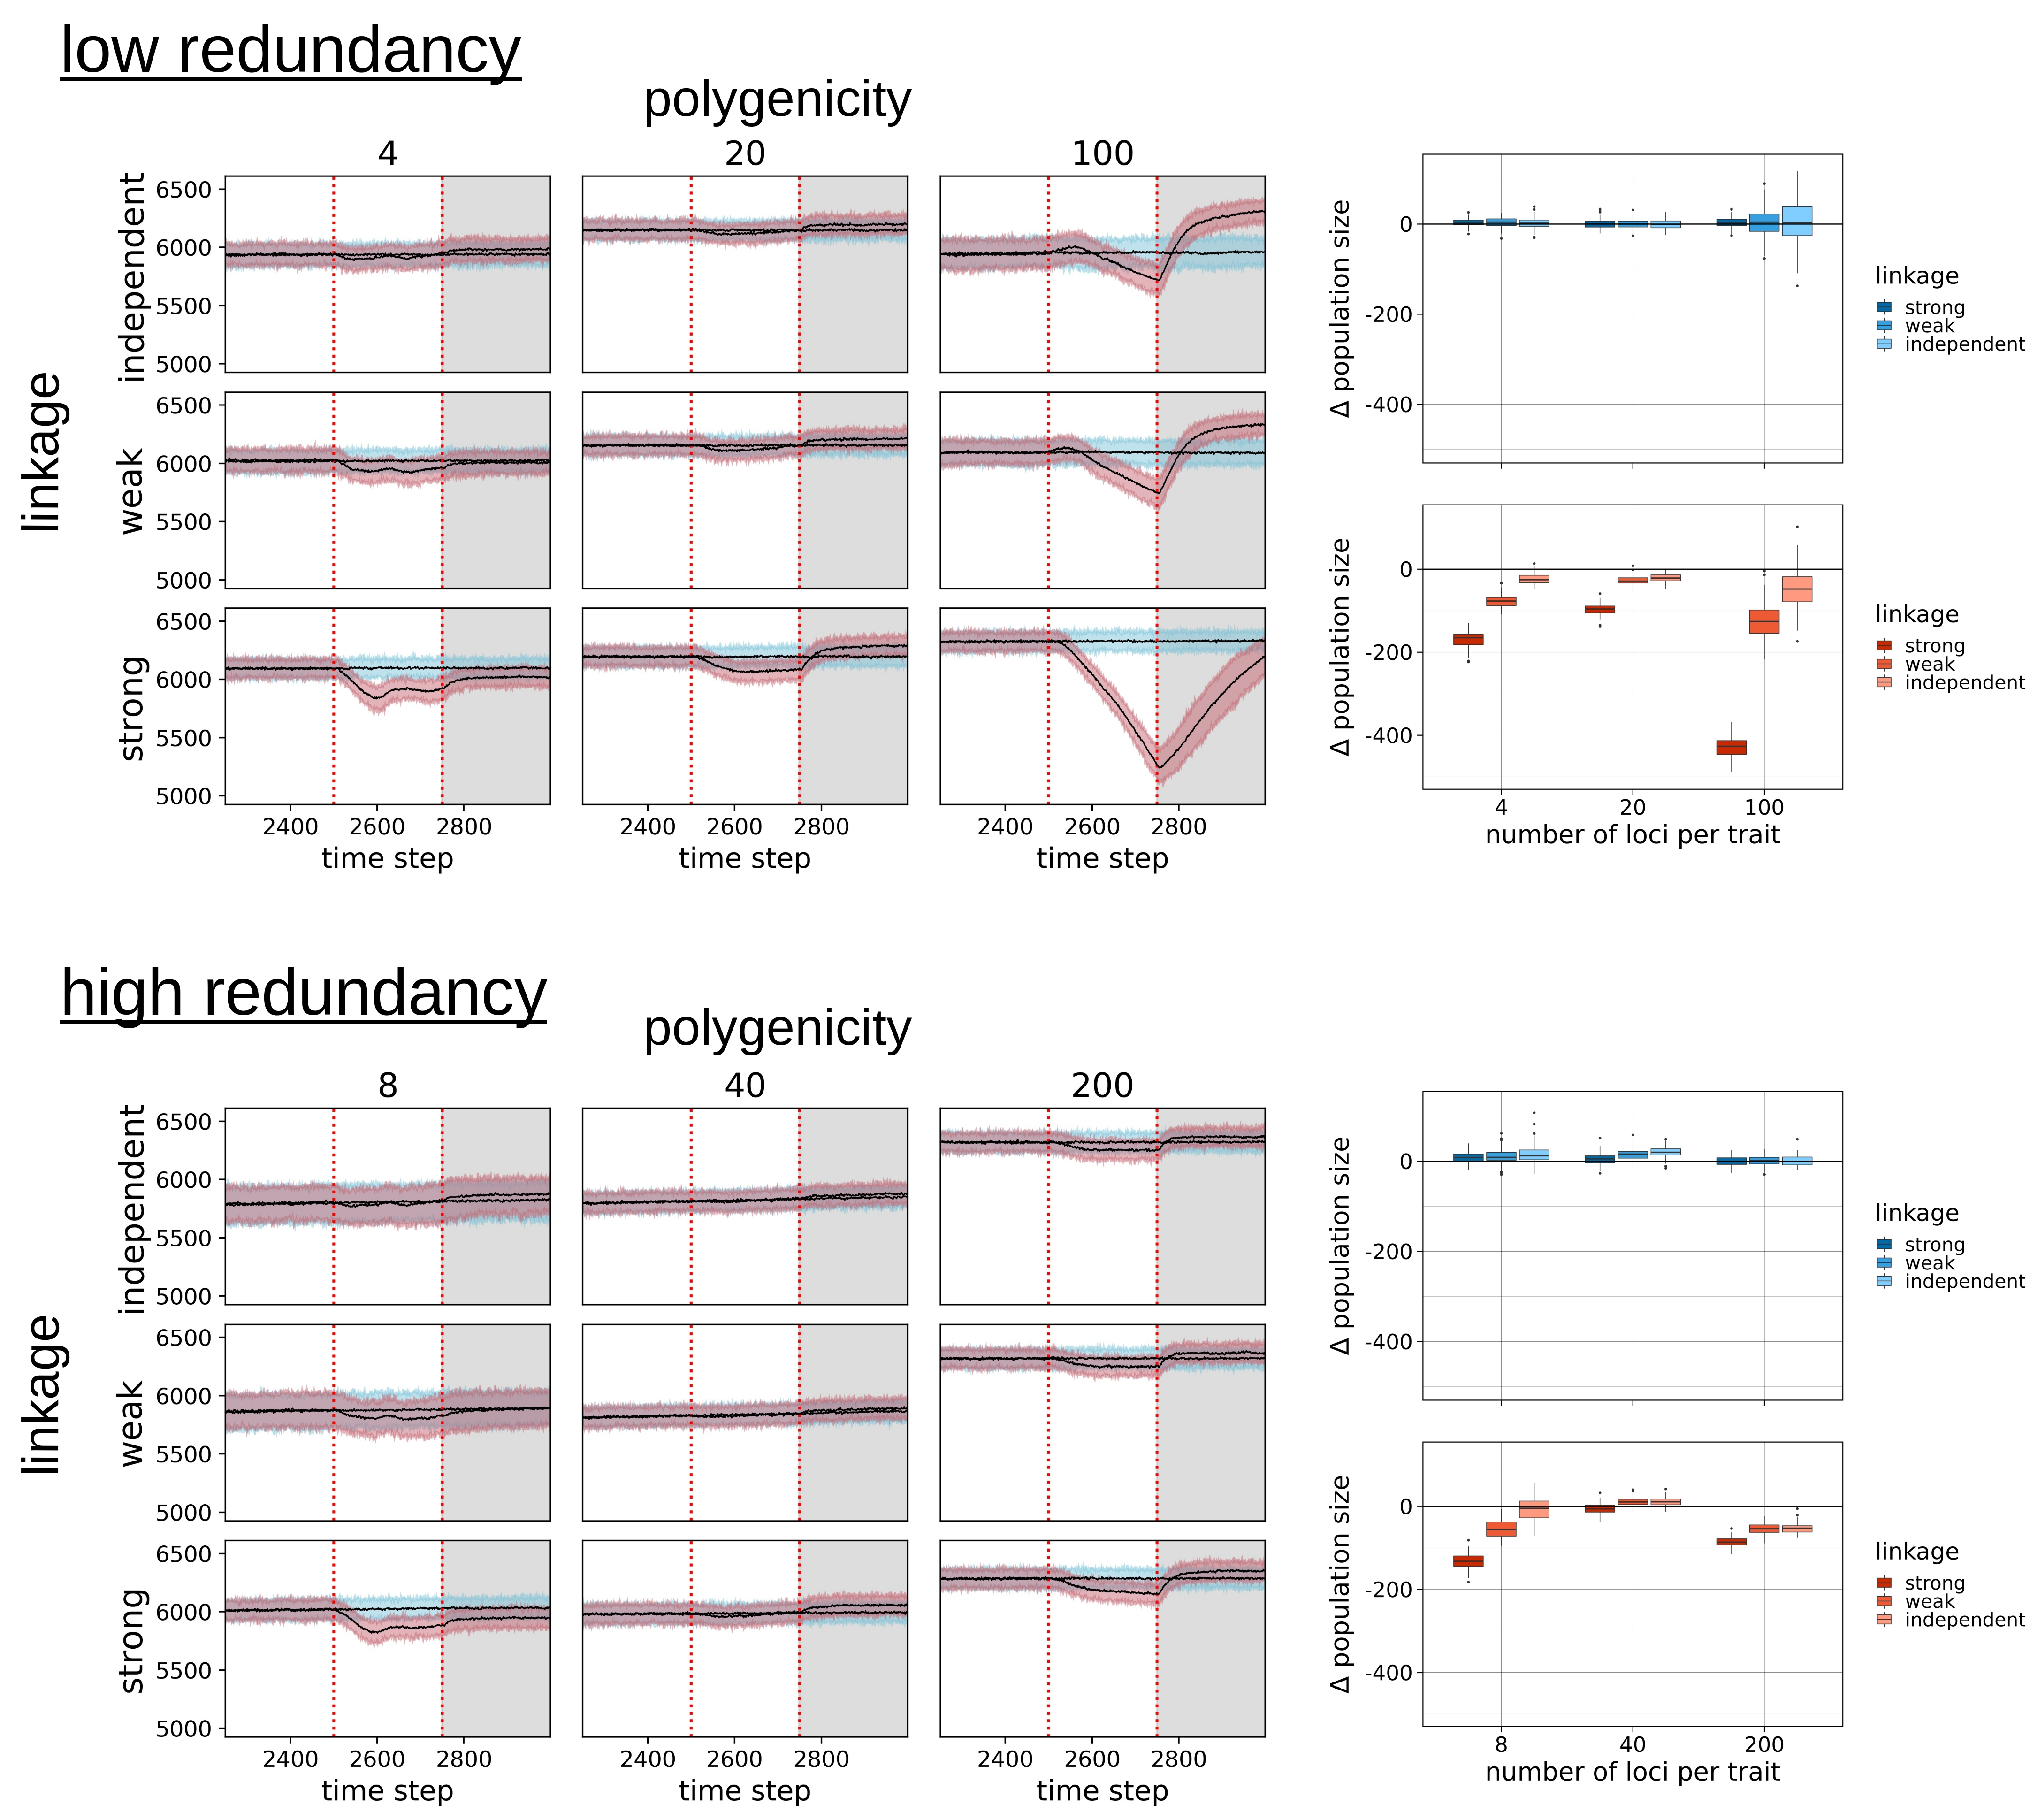
\includegraphics[width=17.8cm]{pub/figs/FIG_S2_Nt_over_time.jpg}
\caption{Left: Population size dynamics for all scenarios during the 250 time steps before the climate change period and the 250 time steps during it (with the two periods divided by a red, dashed vertical line marking the onset of the climate change period). Scenarios are organized as in \ref{fig_2}: top and bottom sections representing low and high redundancy, with rows in each section representing levels of linkage and columns representing polygenicity. Both means (black lines) and variability envelopes (5th percentile to 95th percentile) are shown, with scenario type depicted by color (main scenarios in red, null scenarios in blue). Right: Comparison of climate change-driven changes in mean population size across scenarios. Null scenarios are plotted on the left in blue, and main scenarios are plotted on the right, in red. Within each plot, scenarios are divided by the number of loci per trait (x-axis) and by the strength of linkage (shade, with darker hues representing stronger linkage). Asterisks above each box indicate level of significance (*=0.1, **=0.05, ***=0.005).}
\label{fig:fig_s2}
\end{figure*}

\begin{figure*}
\centering
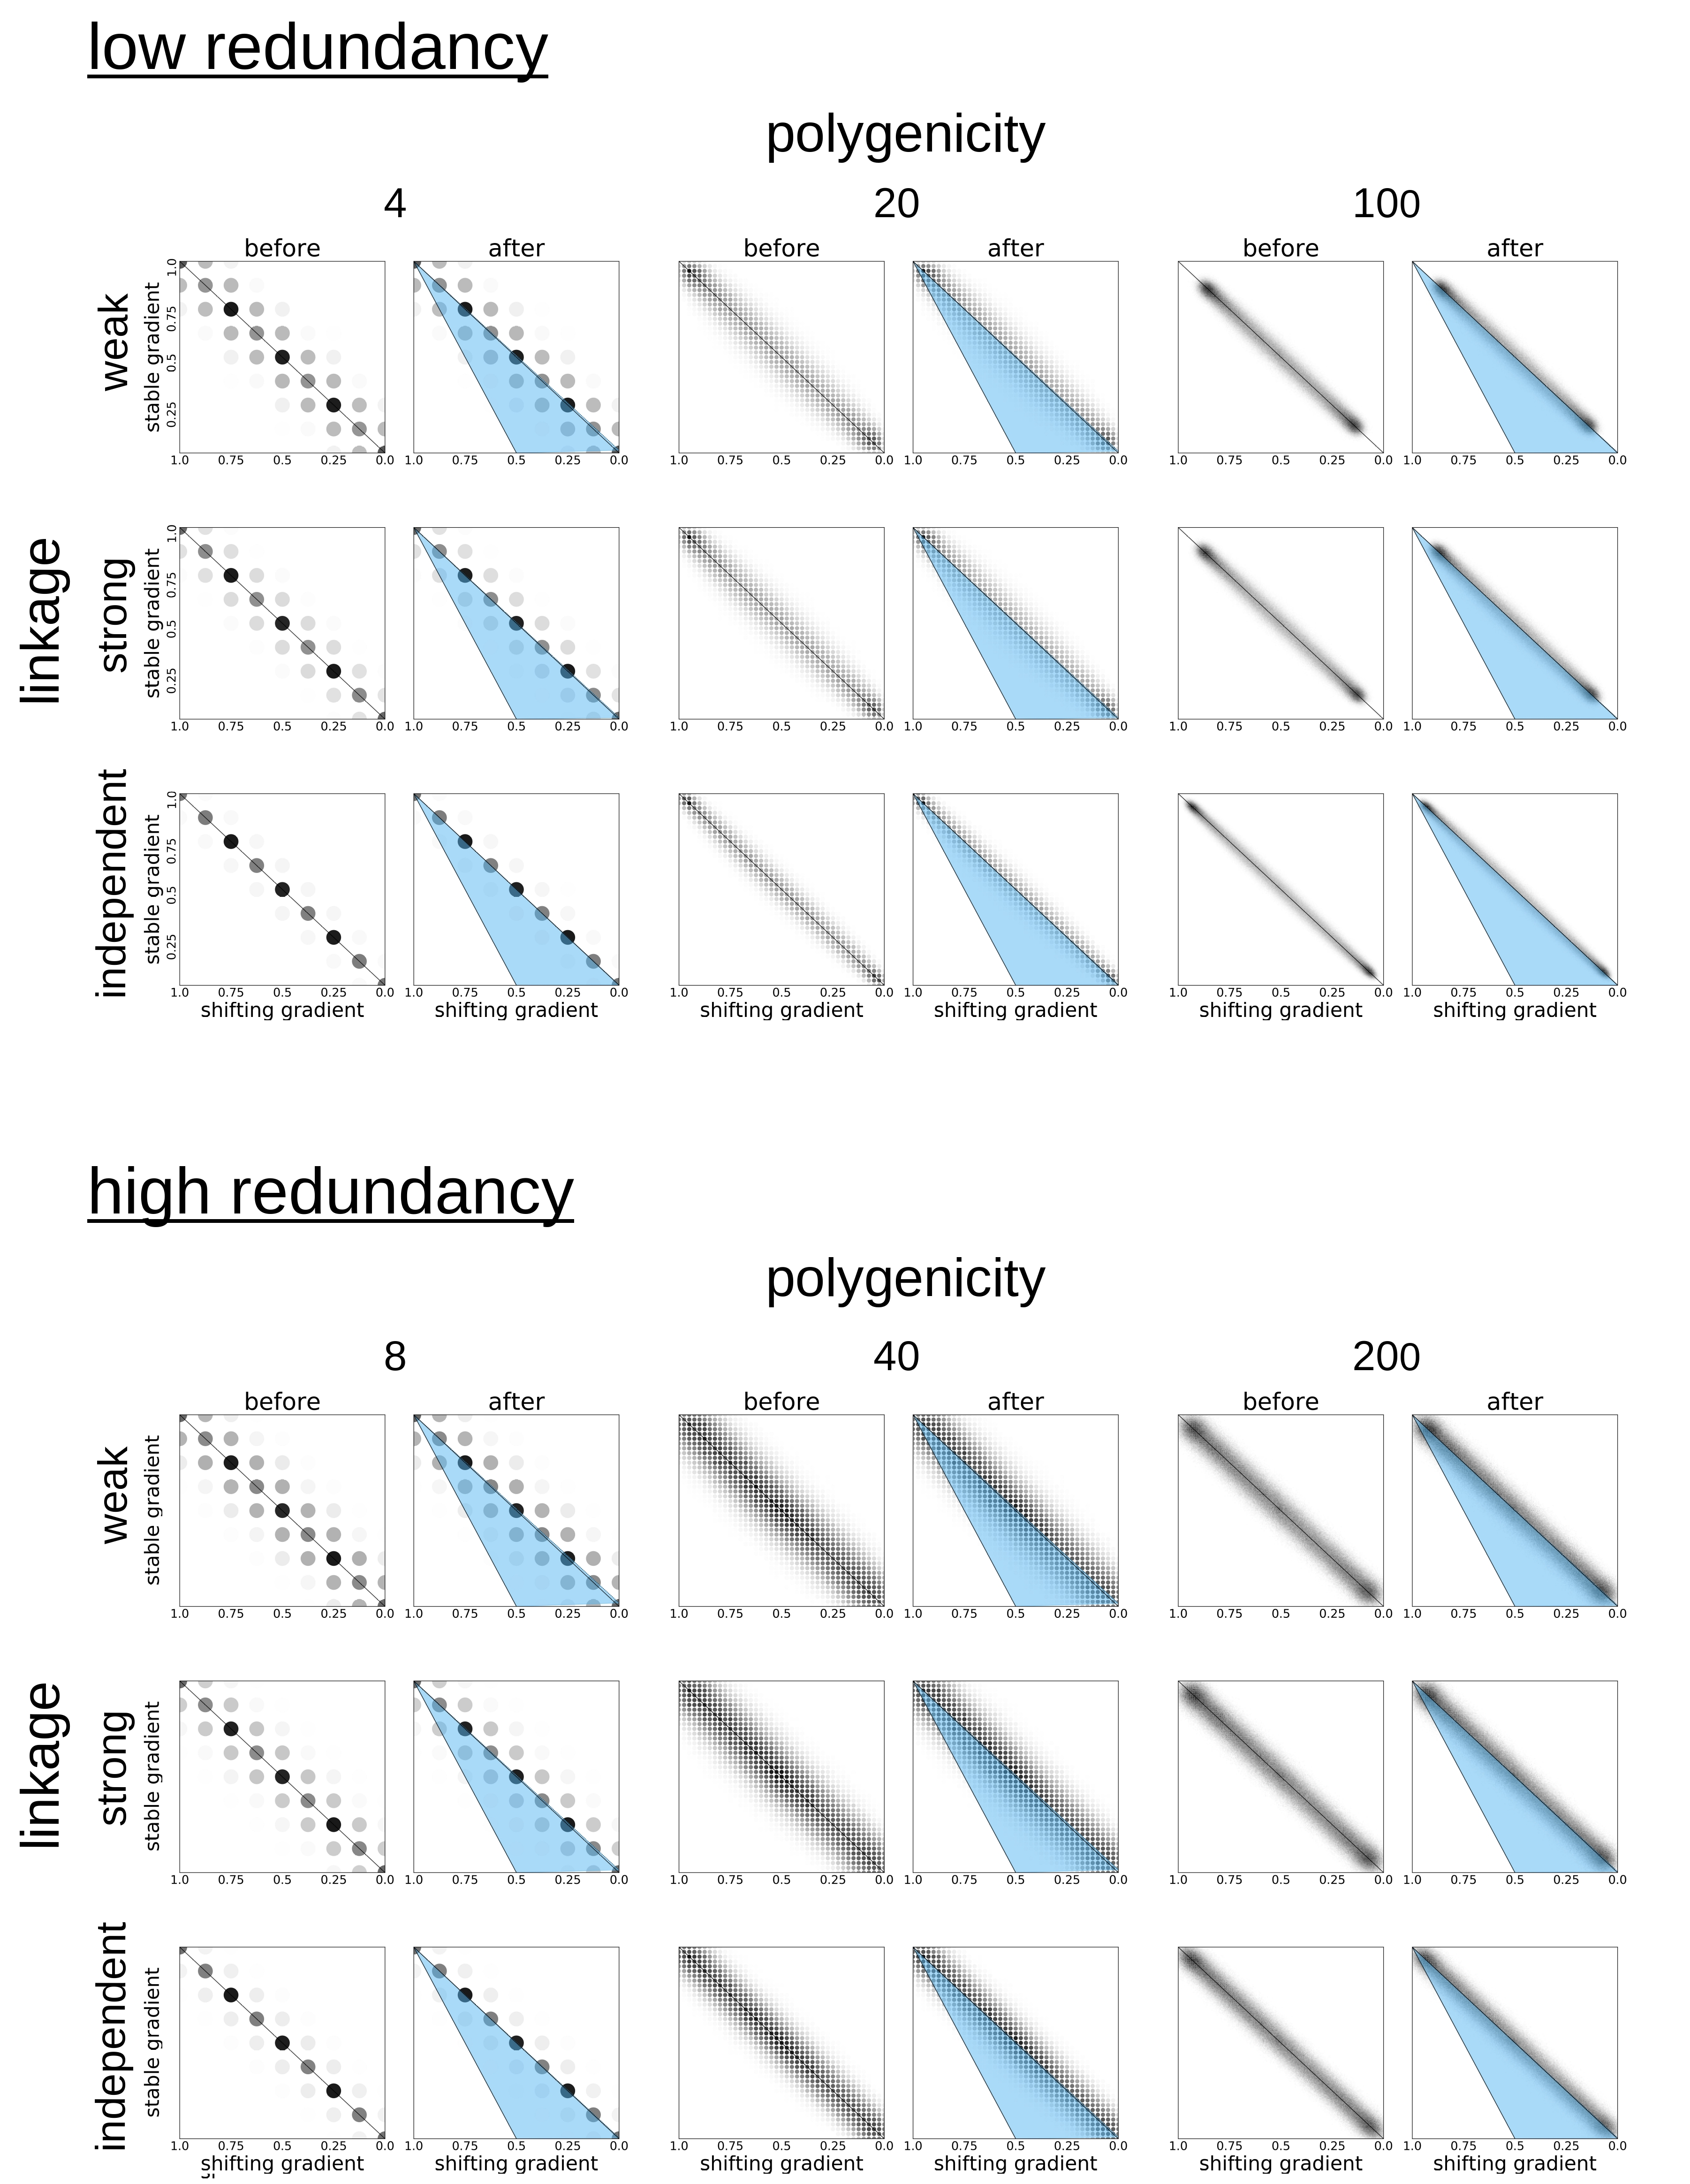
\includegraphics[width=.8\linewidth]{pub/figs/FIG_S3_phenotypic_shift_null.jpg}
    \caption{Maps depicting shifts in population density during climate change for all null simulations. Scenarios are organized as in \ref{fig_2}: top and bottom sections representing low and high redundancy, with rows in each section representing levels of linkage and columns (in before-after pairs) representing polygenicity. As well as showing local extinction in the low-redundancy, high-polygenicity, strong-linkage scenario (bottom right of top section), these maps also show moderate simulation edge effects and density banding in the low-polygenicity scenarios because of the mismatch between environmental and phenotypic resolutions.}
\label{fig:fig_s3}
\end{figure*}

\begin{figure*}
\centering
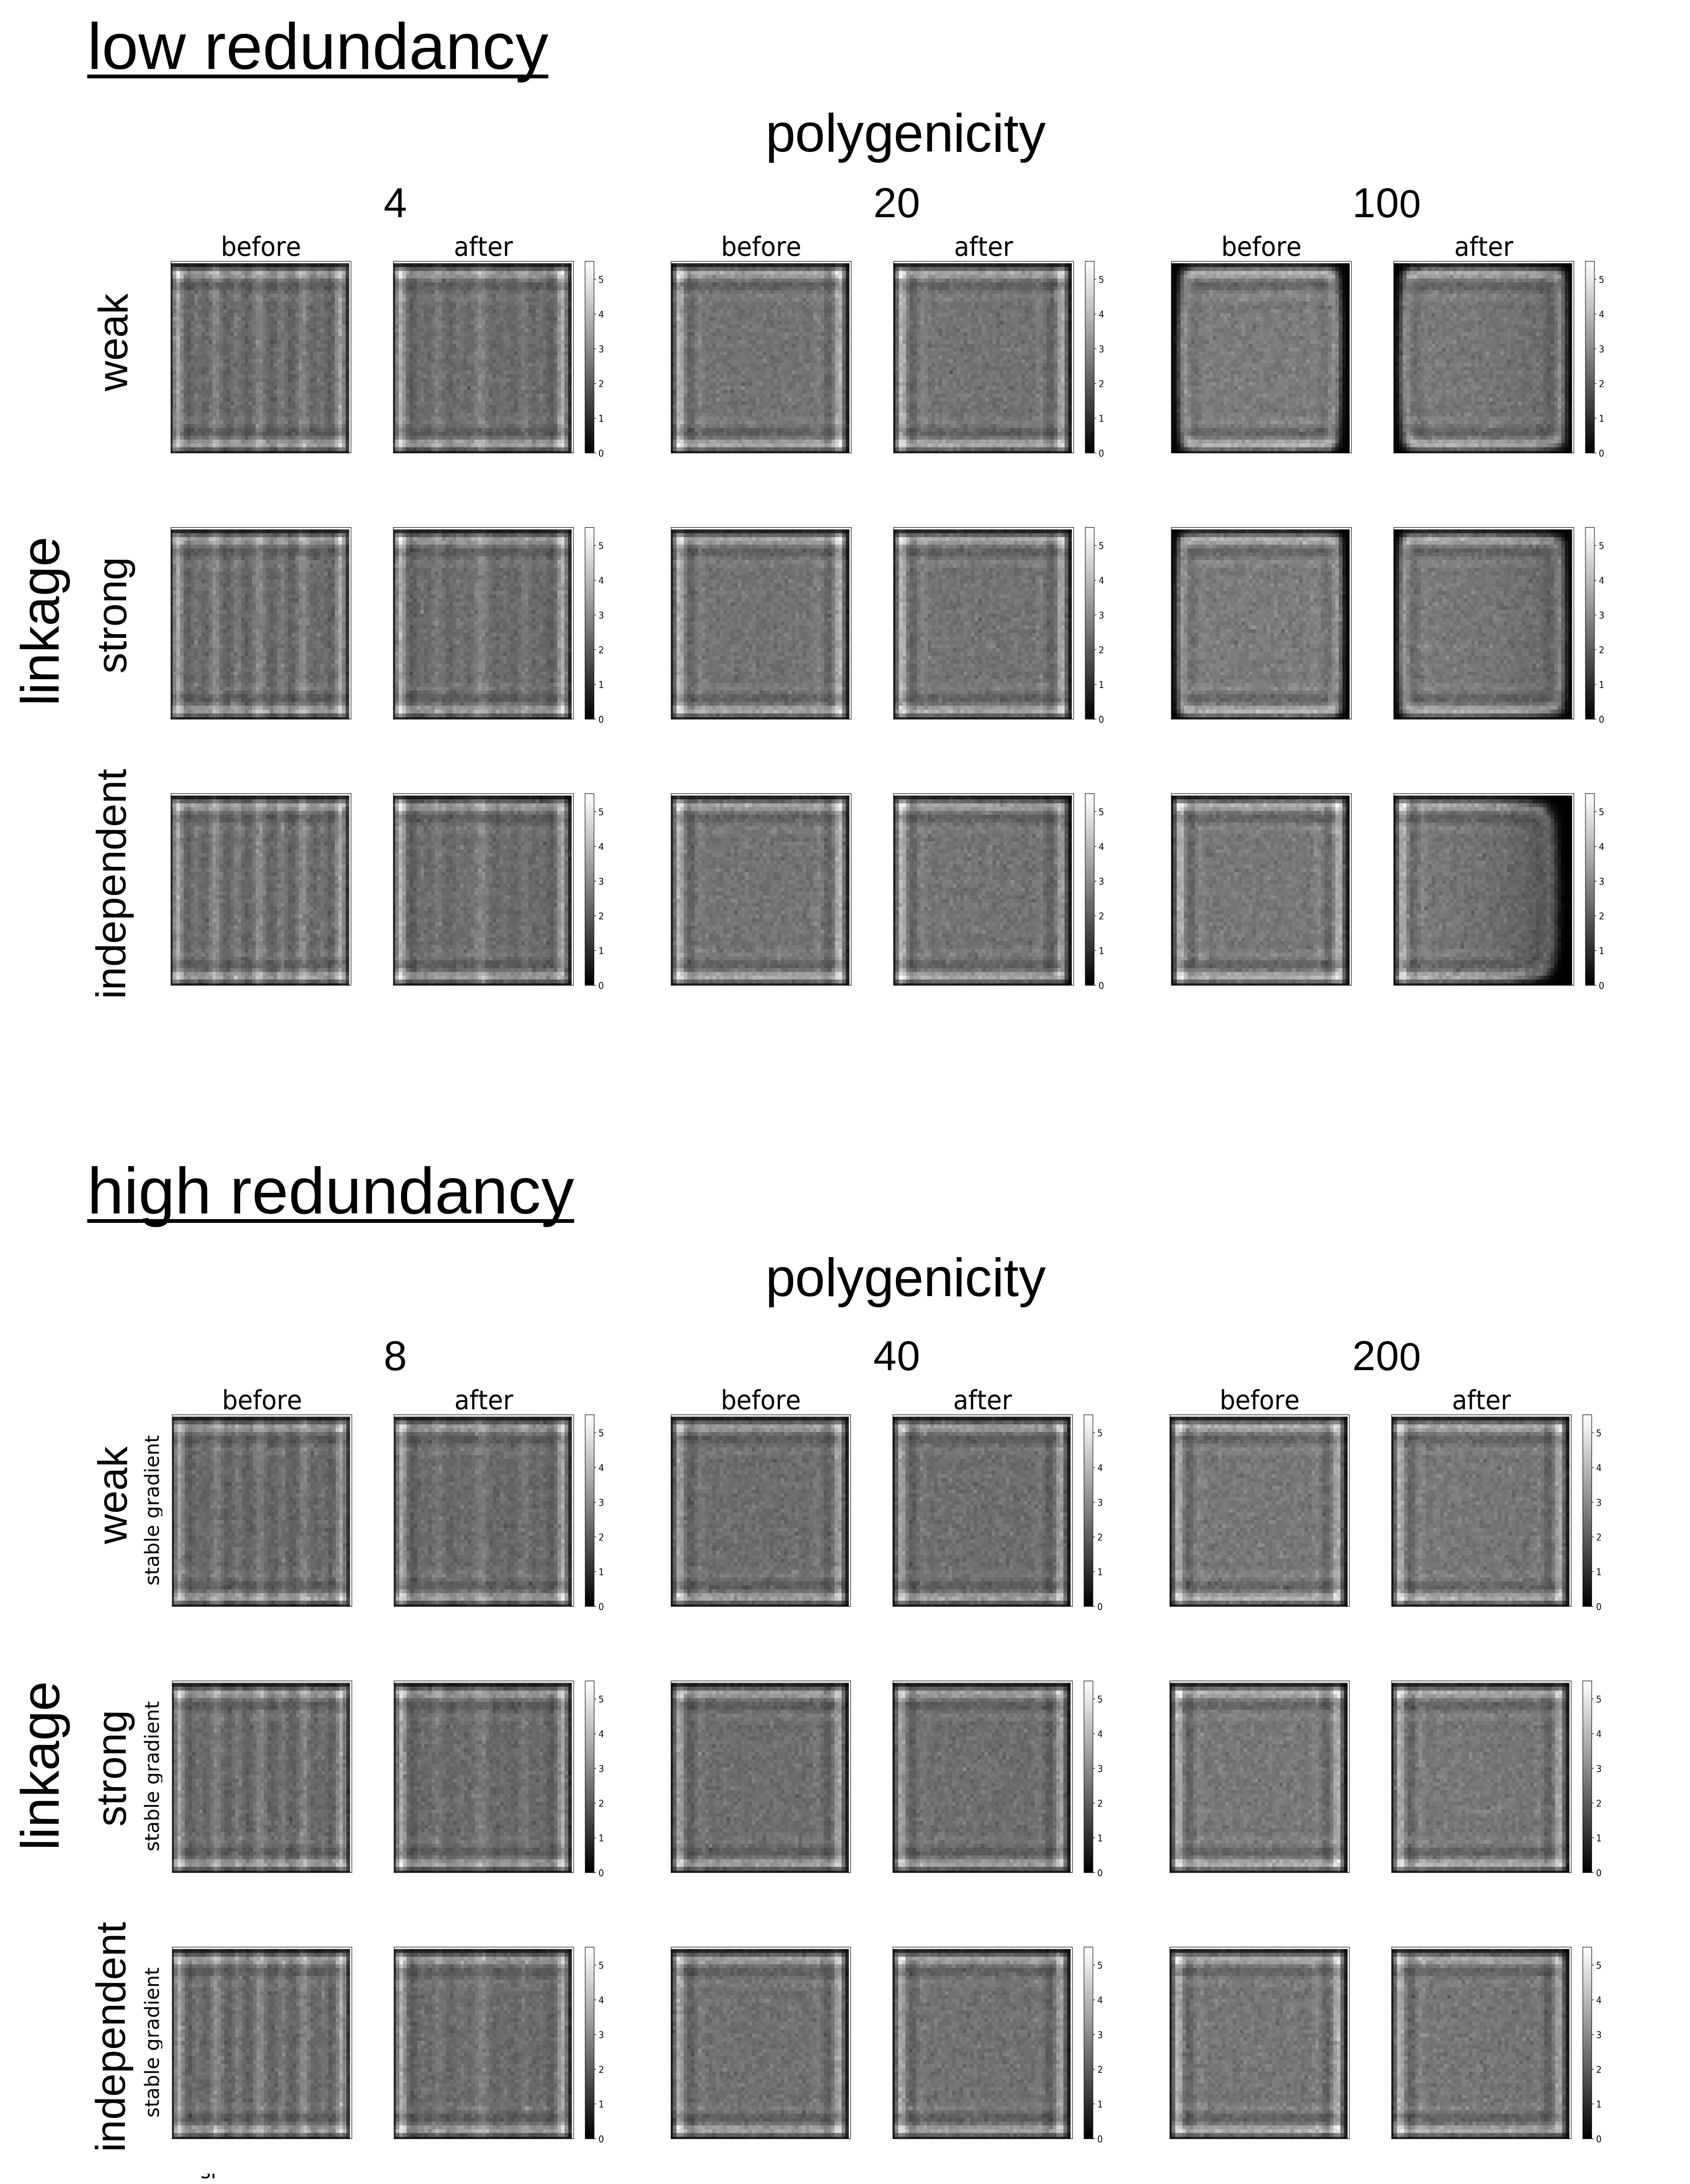
\includegraphics[width=.8\linewidth]{pub/figs/FIG_S4_density_shift.jpg}
\caption{Maps depicting shifts in population density during climate change for all scenarios.}
\label{fig:fig_s4}
\end{figure*}


%%%%%%%%%%%%%%%%%%%%%%%%%%%%%%%%%%%%%%%

\end{document}
